%initialising document, adjust papersize, fontsize and page orientation to your needs
\documentclass[a4paper, fontsize = 8pt, landscape]{scrartcl}
\usepackage{../../../misc_files/LateX/layout_and_colours}
\title{Höhere Mathematik}
\author{Jil Zerndt, Lucien Perret}
\date{January 2025}

\createtitlepagestyle
\createmainpagestyle
\begin{document}
\begin{multicols}{3}
	\thispagestyle{TitlePageStyle}
	\maketitle
	\section{Rechnerarithmetik}

\subsection{Zahlendarstellung}

\begin{definition}{Maschinenzahlen}
Eine maschinendarstellbare Zahl zur Basis $B$ ist ein Element der Menge:
$$M = \{x \in \mathbb{R} \mid x = \pm 0.m_1m_2m_3\ldots m_n \cdot B^{\pm e_1e_2\ldots e_l}\} \cup \{0\}$$
\begin{itemize}
    \item $m_1 \neq 0$ (Normalisierungsbedingung) 
    \item $m_i, e_i \in \{0,1,\ldots,B-1\}$ für $i \neq 0$
    \item $B \in \mathbb{N}, B > 1$ (Basis)
\end{itemize}
\end{definition}

\begin{formula}{Zahlenwert}
Der Wert $\hat{\omega}$ einer Maschinenzahl berechnet sich durch: 
\vspace{-5mm}\\
$$\hat{\omega} = \sum_{i=1}^n m_i B^{\hat{e}-i}, \quad \text{mit} \quad \hat{e} = \sum_{i=1}^l e_i B^{l-i}$$
\end{formula}

\begin{example2}{Werteberechnung} Berechnung einer vierstelligen Zahl zur Basis 4:
    \vspace{-2mm}\\
    \begin{minipage}{0.3\textwidth}
        $$\underbrace{0.3211}_{n=4} \cdot \underbrace{4^{12}}_{l=2}$$
    \end{minipage}
    \begin{minipage}[t]{0.65\textwidth}
        Exponent: $\hat{e} = 1 \cdot 4^1 + 2 \cdot 4^0 = 6$ \vspace{1mm}\\
        Wert: $\hat{\omega} = 3 \cdot 4^3 + 2 \cdot 4^2 + 1 \cdot 4^1 + 1 \cdot 4^0 = 57$
    \end{minipage}
\end{example2}

\begin{concept}{IEEE-754 Standard} definiert zwei wichtige Gleitpunktformate:
\vspace{1mm}\\
\begin{minipage}[t]{0.5\textwidth}
    \textbf{Single Precision} (32 Bit)\\
    Vorzeichen(V): 1 Bit\\
    Exponent(E): 8 Bit (Bias 127)\\
    Mantisse(M): \\ 23 Bit + 1 hidden bit
\end{minipage}
\begin{minipage}[t]{0.48\textwidth}
    \textbf{Double Precision} (64 Bit)\\
    Vorzeichen(V): 1 Bit\\
    Exponent(E): 11 Bit (Bias 1023)\\
    Mantisse(M): \\ 52 Bit + 1 hidden bit
\end{minipage}
\end{concept}

\begin{theorem}{Darstellungsbereich}
Für jedes Gleitpunktsystem existieren:
\begin{itemize}
    \item Grösste darstellbare Zahl: \large{$x_{\text{max}} = (1-B^{-n}) \cdot B^{e_{\text{max}}}$}
    \item \normalsize{Kleinste darstellbare positive Zahl:} \large{$x_{\text{min}} = B^{e_{\text{min}}-1}$}
\end{itemize}
\end{theorem}

\subsection{Approximations- und Rundungsfehler}

\begin{definition}{Fehlerarten}
Sei $\tilde{x}$ eine Näherung des exakten Wertes $x$:
\vspace{1mm}\\
\begin{minipage}[t]{0.35\textwidth}
    \textbf{Absoluter Fehler:}  $$\left|\tilde{x}-x\right|$$
\end{minipage}
\hspace{3mm}
\begin{minipage}[t]{0.5\textwidth}
    \textbf{Relativer Fehler:}  $$\left|\frac{\tilde{x}-x}{x}\right| \text{ bzw. } \frac{|\tilde{x}-x|}{|x|} \text{ für } x \neq 0$$
\end{minipage}
\end{definition}

\begin{lemma}{Maschinengenauigkeit} 
    eps ist die kleinste positive Zahl, für die gilt:
    \vspace{-3mm}\\
\begin{minipage}[t]{0.35\textwidth}
    \textbf{Allgemein:}  $$\text{eps} := \frac{B}{2} \cdot B^{-n}$$
\end{minipage}
\hspace{6mm}
\begin{minipage}[t]{0.35\textwidth}
    \textbf{Dezimal:}  $$\text{eps}_{10} := 5 \cdot 10^{-n}$$
\end{minipage}

\begin{minipage}[t]{0.45\textwidth}
    Sie begrenzt den maximalen relativen Rundungsfehler:
\end{minipage}
\begin{minipage}{0.5\textwidth}
    $$\left|\frac{rd(x)-x}{x}\right| \leq \text{eps}$$
\end{minipage}
\end{lemma}

\begin{corollary}{Rundungseigenschaften}
Für alle $x \in \mathbb{R}$ mit $|x| \geq x_{\text{min}}$ gilt:
\vspace{1mm}\\
\begin{minipage}[t]{0.45\textwidth}
    \textbf{Absoluter Fehler:}  $$|rd(x) - x| \leq \frac{B}{2} \cdot B^{e-n-1}$$
\end{minipage}
\hspace{3mm}
\begin{minipage}[t]{0.35\textwidth}
    \textbf{Relativer Fehler:}  $$\left|\frac{rd(x)-x}{x}\right| \leq \text{eps}$$
\end{minipage}
\end{corollary}

\subsubsection{Fehlerfortpflanzung}

\begin{concept}{Konditionierung}
    Die Konditionszahl $K$ beschreibt die relative Fehlervergrösserung bei Funktionsauswertungen:
    \vspace{1mm}\\
\begin{minipage}{0.3\textwidth}
    \vspace{-2mm}
    $$K := \frac{|f'(x)| \cdot |x|}{|f(x)|}$$
\end{minipage}
\hspace{2mm}
\begin{minipage}{0.6\textwidth}
\begin{itemize}
    \item $K \leq 1$: gut konditioniert
    \item $K > 1$: schlecht konditioniert
    \item $K \gg 1$: sehr schlecht konditioniert
\end{itemize}
\end{minipage}
\end{concept}

\begin{theorem}{Fehlerfortpflanzung}
Für $f$ (differenzierbar) gilt näherungsweise:
\vspace{1mm}\\
\begin{minipage}[t]{0.47\textwidth}
    \textbf{Absoluter Fehler:}  
    \vspace{-2mm}\\
    $$|f(\tilde{x})-f(x)| \approx |f'(x)| \cdot |\tilde{x}-x|$$
\end{minipage}
\hspace{3mm}
\begin{minipage}[t]{0.43\textwidth}
    \textbf{Relativer Fehler:}  
    \vspace{-2mm}\\
    $$\frac{|f(\tilde{x})-f(x)|}{|f(x)|} \approx K \cdot \frac{|\tilde{x}-x|}{|x|}$$
\end{minipage}
\end{theorem}

\begin{KR}{Analyse der Fehlerfortpflanzung einer Funktion}
\begin{enumerate}
    \item Berechnen Sie $f'(x)$
    \item Bestimmen Sie die Konditionszahl $K$
    \item Schätzen Sie den absoluten Fehler ab
    \item Schätzen Sie den relativen Fehler ab
    \item Beurteilen Sie die Konditionierung anhand von $K$
\end{enumerate}
\vspace{1mm}
$$
\begin{aligned}
\underbrace{|f(\tilde{x})-f(x)|}_{\text {absoluter Fehler von } f(x)} & \approx\left|f^{\prime}(x)\right| \cdot \underbrace{|\tilde{x}-x|}_{\text {absoluter Fehler von } x} \\
\underbrace{\frac{|f(\tilde{x})-f(x)|}{|f(x)|}}_{\text {relativer Fehler von } f(x)} & \approx \underbrace{\frac{\left|f^{\prime}(x)\right| \cdot|x|}{|f(x)|}}_{\text {Konditionszahl } K} . \quad \underbrace{\frac{|\tilde{x}-x|}{|x|}}_{\text { relativer Fehler von } x }
\end{aligned}
$$
\end{KR}

\raggedcolumns

\begin{example2}{Fehleranalyse}Beispiel: Fehleranalyse von $f(x)=\sin(x)$
\begin{enumerate}
    \item $f'(x) = \cos(x)$
    \item $K = \frac{|x\cos(x)|}{|\sin(x)|}$
    \item Für $x \to 0$: $K \to 1$ (gut konditioniert)
    \item Für $x \to \pi$: $K \to \infty$ (schlecht konditioniert)
    \item Der absolute Fehler wird nicht vergrössert, da $|\cos(x)| \leq 1$
\end{enumerate}
\end{example2}

\subsubsection{Praktische Fehlerquellen der Numerik}

\begin{concept}{Kritische Operationen} häufigste Fehlerquellen:
\begin{itemize}
    \item Auslöschung bei Subtraktion ähnlich großer Zahlen
    \item Überlauf (overflow) bei zu großen Zahlen
    \item Unterlauf (underflow) bei zu kleinen Zahlen
    \item Verlust signifikanter Stellen durch Rundung
\end{itemize}
\end{concept}



\begin{KR}{Vermeidung von Auslöschung}
\begin{enumerate}
    \item Identifizieren Sie Subtraktionen ähnlich großer Zahlen
    \item Suchen Sie nach algebraischen Umformungen
    \item Prüfen Sie alternative Berechnungswege
    \item Verwenden Sie Taylorentwicklungen für kleine Werte
\end{enumerate}
\end{KR}

\begin{example2}{Auslöschung} bei der Berechnung von $\sqrt{x^2 + 1} - 1$:
    \vspace{1mm}\\
    Für kleine $x$ führt die direkte Berechnung zu Auslöschung:
    \vspace{1mm}\\
    Für $x = 10^{-8}$: $\sqrt{10^{-16} + 1} - 1 \approx 1.000000000 - 1 = 0$
    \vspace{1mm}\\
    Korrekte Lösung durch Umformung: $\sqrt{x^2 + 1} - 1 = \frac{x^2}{\sqrt{x^2 + 1} + 1}$
\end{example2}

\begin{remark2}{Auslöschung}
    Bei der Subtraktion fast gleich großer Zahlen können signifikante Stellen verloren gehen. Beispiel:
    \begin{itemize}
        \item $1.234567 - 1.234566 = 0.000001$
        \item Aus 7 signifikanten Stellen wird 1 signifikante Stelle
    \end{itemize}
\end{remark2}

\subsubsection{Analyse von Algorithmen}

\begin{formula}{Fehlerakkumulation}
Bei $n$ aufeinanderfolgenden Operationen mit relativen Fehlern $\leq \varepsilon$ gilt für den Gesamtfehler:
\begin{itemize}
    \item Best case: $\mathcal{O}(n\varepsilon)$ bei gleichverteilten Fehlern
    \item Worst case: $\mathcal{O}(2^n\varepsilon)$ bei systematischen Fehlern
\end{itemize}
\end{formula}

\begin{concept}{Numerische Stabilität eines Algorithmus}
\begin{itemize}
    \item Kleine Eingabefehler führen zu kleinen Ausgabefehlern
    \item Rundungsfehler akkumulieren sich nicht übermäßig 
    \item Konditionszahl des Problems wird nicht künstlich verschlechtert
\end{itemize}
\end{concept}

\begin{examplecode}{Instabilität} bei rekursiver Berechnung: (Fibonacci-Zahlen)
\begin{lstlisting}[language=Python, style=basesmol]
def fib(n):
    if n <= 1:
        return n
    return fib(n-1) + fib(n-2)
\end{lstlisting}
Exponentielles Wachstum der Operationen $\rightarrow$ Fehlerfortpflanzung
\end{examplecode}

\begin{KR}{Stabilitätsanalyse}
Schritte zur Analyse der numerischen Stabilität:
\begin{enumerate}
    \item Bestimmen Sie kritische Operationen
    \item Schätzen Sie Rundungsfehler pro Operation ab
    \item Analysieren Sie die Fehlerfortpflanzung
    \item Berechnen Sie die worst-case Fehlerschranke
    \item Vergleichen Sie alternative Implementierungen
\end{enumerate}
\end{KR}

\subsubsection{Praktische Implementierungen}

\begin{definition}{Implementierungsgenauigkeit eines Algorithmus}
\begin{itemize}
    \item Relative Genauigkeit der Ausgabe
    \item Maximale Anzahl korrekter Dezimalstellen
    \item Stabilität gegenüber Eingabefehlern
\end{itemize}
\end{definition}

\begin{KR}{Robuste Implementierung von Algorithmen}
\begin{enumerate}
    \item Verwenden Sie stabile Grundoperationen
    \item Vermeiden Sie Differenzen ähnlich großer Zahlen
    \item Prüfen Sie auf Über- und Unterlauf
    \item Implementieren Sie Fehlerkontrollen
    \item Dokumentieren Sie numerische Einschränkungen
\end{enumerate}
\end{KR}

\begin{examplecode}{Robuste Implementation} Beispiel: Quadratische Gleichung
\begin{lstlisting}[language=Python, style=basesmol]
def quadratic_stable(a, b, c):
    # ax^2 + bx + c = 0
    if a == 0:
        return [-c/b] if b != 0 else []
        
    # Calculate discriminant
    disc = b*b - 4*a*c
    if disc < 0:
        return []

    # Choose numerically stable formula
    if b >= 0:
        q = -0.5*(b + sqrt(disc))
    else:
        q = -0.5*(b - sqrt(disc))
    x1 = q/a
    x2 = c/(q)

    return sorted([x1, x2])
\end{lstlisting}
\end{examplecode}

	
	\raggedcolumns
	

	\section{Numerische Lösung von Nullstellenproblemen}

\begin{lemma}{Nullstellensatz von Bolzano}
Sei $f:[a,b] \rightarrow \mathbb{R}$ stetig. Falls 
\vspace{-1mm}\\
$$f(a) \cdot f(b) < 0$$ 
\vspace{-3mm}\\
dann existiert mindestens eine Nullstelle $\xi \in (a,b)$.
\end{lemma}

\begin{KR}{Systematisches Vorgehen bei Nullstellenproblemen}
    \begin{itemize}
        \item Newton-Verfahren: wenn Ableitung leicht berechenbar
        \item Sekantenverfahren: wenn Ableitung schwierig
        \item Fixpunktiteration: wenn geeignete Umformung möglich
    \end{itemize}
\end{KR}

\begin{remark}
    NSP: Nullstellenproblem, NS: Nullstelle
\end{remark}



\subsubsection{Fixpunktiteration}

\begin{definition}{Fixpunktgleichung}
ist eine Gleichung der Form: $F(x)=x$\\
Die Lösungen $\bar{x}$, für die $F(\bar{x})=\bar{x}$ erfüllt ist, heissen Fixpunkte.
\end{definition}

\begin{concept}{Grundprinzip der Fixpunktiteration}
sei $F:[a,b] \rightarrow \mathbb{R}$ mit $x_0 \in [a,b]$ 
\vspace{-6mm}\\
$$\text{Die rekursive Folge }x_{n+1} \equiv F(x_n), \quad n=0,1,2,\ldots$$
\vspace{-4mm}\\
heisst Fixpunktiteration von $F$ zum Startwert $x_0$.
\end{concept}

\begin{theorem}{Konvergenzverhalten}\\
Sei $F:[a,b] \rightarrow \mathbb{R}$ mit stetiger Ableitung $F'$ und $\bar{x} \in [a,b]$ ein Fixpunkt von $F$. Dann gilt für die Fixpunktiteration $x_{n+1}=F(x_n)$:
\vspace{1mm}\\
\begin{minipage}[t]{0.45\textwidth}
    \textbf{Anziehender Fixpunkt:}
    \vspace{-3mm}\\
    $$|F'(\bar{x})| < 1$$
    \vspace{-4mm}\\
    $x_n$ konvergiert gegen $\bar{x}$,\\
    falls $x_0$ nahe genug bei $\bar{x}$
\end{minipage}
\hspace{3mm}
\begin{minipage}[t]{0.45\textwidth}
    \textbf{Abstossender Fixpunkt:}
    \vspace{-3mm}\\
    $$|F'(\bar{x})| > 1$$
    \vspace{-4mm}\\
    $x_n$ konvergiert für keinen\\
    Startwert $x_0 \neq \bar{x}$
\end{minipage}
\end{theorem}

\begin{lemma}{Banachscher Fixpunktsatz}
$F:[a,b] \rightarrow [a,b]$ und $\exists$ Konstante $\alpha$:
\begin{itemize}
    \item $0 < \alpha < 1$ (Lipschitz-Konstante)
    \item $|F(x)-F(y)| \leq \alpha|x-y|$ für alle $x,y \in [a,b]$
\end{itemize}
\vspace{2mm}


\begin{minipage}[t]{0.35\textwidth}
    Dann gilt:
\begin{itemize}
    \item $F$ hat genau einen Fixpunkt $\bar{x}$ in $[a,b]$
    \item Die Fixpunktiteration konvergiert gegen $\bar{x}$ für alle $x_0 \in [a,b]$
\end{itemize}
\end{minipage}
\hspace{2mm}
\begin{minipage}[t]{0.55\textwidth}
    \textbf{Fehlerabschätzungen}:
    \vspace{-2mm}\\
    $$\textbf{a-priori: } |x_n-\bar{x}| \leq \frac{\alpha^n}{1-\alpha} \cdot |x_1-x_0|$$
    $$\textbf{a-posteriori: } |x_n-\bar{x}| \leq \frac{\alpha}{1-\alpha} \cdot |x_n-x_{n-1}|$$
\end{minipage}
\end{lemma}

\begin{KR}{Konvergenznachweis für Fixpunktiteration}
\begin{enumerate}
    \item Bringe die Gleichung in Fixpunktform: $f(x)=0 \Rightarrow x = F(x)$
    \item Prüfe, ob $F$ das Intervall $[a,b]$ in sich abbildet:
    \begin{itemize}
        \item Wähle geeignetes Intervall ($[a,b]$ $F(a) \geq a$ und $F(b) \leq b$)
    \end{itemize}
    \item Bestimme die Lipschitz-Konstante $\alpha$: $\rightarrow$ Berechne $F'(x)$
    \begin{itemize}
        \item Finde $\alpha = \max_{x \in [a,b]} |F'(x)|$ und prüfe $\alpha < 1$
    \end{itemize}
\end{enumerate}

\begin{minipage}[t]{0.5\textwidth}
    4. Berechnen Sie die nötigen \\Iterationen für Genauigkeit tol:
\end{minipage}
\begin{minipage}[t]{0.4\textwidth}
    \vspace{-3mm}
$$n \geq \frac{\ln(\frac{tol \cdot (1-\alpha)}{|x_1-x_0|})}{\ln \alpha}$$
\end{minipage}
\end{KR}

\begin{example2}{Fixpunktiteration} Nullstellen von $f(x)=e^x - x - 2$

Umformung in Fixpunktform: $x = \ln(x+2)$, also $F(x)=\ln(x+2)$
\begin{enumerate}
    \item $F'(x) = \frac{1}{x+2}$ monoton fallend
    \item Für $I=[1,2]$: $F(1)=1.099 > 1$, $F(2)=1.386 < 2$
    \item $\alpha = \max_{x \in [1,2]} |\frac{1}{x+2}| = \frac{1}{3} < 1$
    \item Konvergenz für Startwerte in $[1,2]$ gesichert
    \item Für Genauigkeit $10^{-6}$ benötigt: $n \geq 12$ Iterationen
\end{enumerate}
\end{example2}



\subsubsection{Newton-Verfahren}

\begin{concept}{Grundprinzip Newton-Verfahren}
    \vspace{-2mm}\\
\begin{minipage}[t]{0.6\textwidth}
    Approximation der NS durch \\ sukzessive Tangentenberechnung:
\end{minipage}
\begin{minipage}{0.3\textwidth}
    \vspace{-3mm}
    $$x_{n+1} = x_n - \frac{f(x_n)}{f'(x_n)}$$
\end{minipage}
\vspace{-2mm}\\
\begin{minipage}[t]{0.6\textwidth}
    Konvergiert, wenn für alle $x$ im \\ relevanten Intervall gilt:
\end{minipage}
\begin{minipage}{0.3\textwidth}
    \vspace{-3mm}
    $$\left|\frac{f(x) \cdot f''(x)}{[f'(x)]^2}\right| < 1$$
\end{minipage}
\end{concept}

\begin{KR}{Newton-Verfahren anwenden}
\begin{enumerate}
    \item Funktion $f(x)$ und Ableitung $f'(x)$ aufstellen
    \item Geeigneten Startwert $x_0$ nahe der Nullstelle wählen
    \begin{itemize}
        \item Prüfen, ob $f'(x_0) \neq 0$
    \end{itemize}
    \item Iterieren bis zur gewünschten Genauigkeit:
    $x_{n+1} = x_n - \frac{f(x_n)}{f'(x_n)}$
    \item Abbruchkriterien prüfen:
    \begin{itemize}
        \item Funktionswert: $|f(x_n)| < \epsilon_1$
        \item Änderung aufeinanderfolgenden Werte: $|x_{n+1}-x_n| < \epsilon_2$
        \item Maximale Iterationszahl nicht überschritten
    \end{itemize}
\end{enumerate}
\end{KR}

\begin{example2}{Newton-Verfahren} Nullstellen von $f(x)=x^2-2$\\
Ableitung: $f'(x) = 2x$, Startwert $x_0 = 1$
\vspace{1mm}\\
\begin{minipage}[t]{0.65\textwidth}
    \vspace{-3mm}
    \begin{enumerate}
        \item $x_1 = 1 - \frac{1^2-2}{2 \cdot 1} = 1.5$
        \item $x_2 = 1.5 - \frac{1.5^2-2}{2 \cdot 1.5} = 1.4167$
        \item $x_3 = 1.4167 - \frac{1.4167^2-2}{2 \cdot 1.4167} = 1.4142$
    \end{enumerate}
\end{minipage}
\begin{minipage}[t]{0.3\textwidth}
    $\rightarrow$ Konvergenz \\ gegen $\sqrt{2}$ nach \\ wenigen Schritten
\end{minipage}
\end{example2}

\begin{theorem}{Vereinfachtes Newton-Verfahren}\\
    \begin{minipage}{0.5\textwidth}
        Alternative Variante mit \\ konstanter Ableitung:
    \end{minipage}
    \begin{minipage}{0.25\textwidth}
        \vspace{-5mm}
        $$x_{n+1} = x_n - \frac{f(x_n)}{f'(x_0)}$$
    \end{minipage}
    \vspace{1mm}\\
    Konvergiert langsamer, aber benötigt weniger Rechenaufwand.
\end{theorem}

\begin{concept}{Sekantenverfahren}\\
    Alternative zum Newton-Verfahren ohne Ableitungsberechnung. Verwendet zwei Punkte $(x_{n-1}, f(x_{n-1}))$ und $(x_n, f(x_n))$:
    \vspace{-2mm}\\
    $$x_{n+1} = x_n - \frac{x_n-x_{n-1}}{f(x_n)-f(x_{n-1})} \cdot f(x_n)$$
    \vspace{-3mm}\\
    Benötigt zwei Startwerte $x_0$ und $x_1$.
\end{concept}


\begin{example2}{Sekantenverfahren} Nullstellen von $f(x)=x^2-2$\\
    %TODO: check if this is correct and/or relevant - either correct or replace with better example
Startwerte $x_0 = 1$ und $x_1 = 2$
\vspace{1mm}\\
\begin{minipage}[t]{0.65\textwidth}
    \vspace{-3mm}
    \begin{enumerate}
        \item $x_2 = 1 - \frac{1-2}{1^2-2} \cdot 1 = 1.5$
        \item $x_3 = 1.5 - \frac{1.5-1}{1.5^2-2} \cdot 1.5 = 1.4545$
        \item $x_4 = 1.4545 - \frac{1.4545-1.5}{1.4545^2-2} \cdot 1.4545 = 1.4143$
    \end{enumerate}
\end{minipage}
\hspace{2mm}
\begin{minipage}[t]{0.28\textwidth}
    $\rightarrow$ Konvergenz\\ gegen $\sqrt{2}$ nach \\wenigen Schritten
\end{minipage}
\end{example2}


\subsubsection{Fehlerabschätzung}



\begin{KR}{Fehlerabschätzung für Nullstellen}\\
So schätzen Sie den Fehler einer Näherungslösung ab:
\begin{enumerate}
    \item Sei $x_n$ der aktuelle Näherungswert
    \item Wähle Toleranz $\epsilon > 0$
    \item Prüfe Vorzeichenwechsel: $f(x_n-\epsilon) \cdot f(x_n+\epsilon) < 0$
    \item Falls ja: Nullstelle liegt in $(x_n-\epsilon, x_n+\epsilon)$
    \item Damit gilt: $|x_n-\xi| < \epsilon$
\end{enumerate}
\end{KR}


\begin{example2}{Praktische Fehlerabschätzung} Fehlerbestimmung bei $f(x)=x^2-2$
    \vspace{-1mm}\\
    \begin{minipage}[t]{0.6\textwidth}
        \vspace{-3mm}
        \begin{enumerate}
            \item Näherungswert: $x_3 = 1.4142157$
            \item Mit $\epsilon = 10^{-5}$:
            \item $f(x_3-\epsilon) = 1.4142057^2 - 2 < 0$
            \item $f(x_3+\epsilon) = 1.4142257^2 - 2 > 0$
        \end{enumerate}
    \end{minipage}
    \begin{minipage}[t]{0.35\textwidth}
        \textbf{Also}: $|x_3-\sqrt{2}| < 10^{-5}$
        \vspace{-1mm}\\
        $\rightarrow$ Nullstelle liegt in $(1.4142057, 1.4142257)$
    \end{minipage}
\end{example2}

\subsection{Konvergenzverhalten}

\begin{definition}{Konvergenzordnung}
    Sei $(x_n)$ eine gegen $\bar{x}$ konvergierende Folge. \\
    Die Konvergenzordnung $q \geq 1$ ist definiert durch:
    \vspace{-2mm}\\
    $$|x_{n+1}-\bar{x}| \leq c \cdot |x_n-\bar{x}|^q$$
    wo $c > 0$ eine Konstante. Für $q = 1$ muss zusätzl. $c < 1$ gelten.
\end{definition}

\begin{theorem}{Konvergenzordnungen der Verfahren} Konvergenzgeschwindigkeiten
    \vspace{-2mm}\\
    \textbf{Newton-Verfahren:} Quadratische Konvergenz: $q = 2$
    \vspace{1mm}\\
    \textbf{Vereinfachtes Newton:} Lineare Konvergenz: $q = 1$
    \vspace{1mm}\\
    \textbf{Sekantenverfahren:} Superlineare Konvergenz: $q = \frac{1+\sqrt{5}}{2} \approx 1.618$
\end{theorem}

\begin{example2}{Konvergenzgeschwindigkeit} Vergleich der Verfahren:
    \vspace{1mm}\\
    Startwert $x_0 = 1$, Funktion $f(x) = x^2 - 2$, Ziel: $\sqrt{2}$
    \begin{center}
    \begin{tabular}{l|c|c|c}
    n & Newton & Vereinfacht & Sekanten \\\hline
    1 & 1.5000000 & 1.5000000 & 1.5000000\\
    2 & 1.4166667 & 1.4500000 & 1.4545455\\
    3 & 1.4142157 & 1.4250000 & 1.4142857\\
    4 & 1.4142136 & 1.4125000 & 1.4142136
    \end{tabular}
    \end{center}
\end{example2}

\subsection{Implementationen}

\begin{examplecode}{Fixpunktiteration}
\begin{lstlisting}[language=Python, style=basesmol]
# Einfache Version
def fixed_point_iter(f, x0, tol=1e-6, max_iter=100):
    x = x0
    for i in range(max_iter):
        x_new = f(x)
        if abs(x_new - x) < tol:
            return x_new, i+1
        x = x_new
    raise ValueError("Keine Konvergenz")

# Optimierte Version mit Fehlerschaetzung
def fixed_point_iter_opt(f, x0, tol=1e-6, max_iter=100):
    x = x0
    alpha = None  # Schaetzung fuer Lipschitz-Konstante
    for i in range(max_iter):
        x_new = f(x)
        dx = abs(x_new - x)
        
        # Lipschitz-Konstante schaetzen
        if i > 0 and dx > 0:
            alpha_new = dx / dx_old
            if alpha is None or alpha_new > alpha:
                alpha = alpha_new
        
        # A-posteriori Fehlerabschaetzung
        if alpha is not None and alpha < 1:
            error = alpha * dx / (1 - alpha)
            if error < tol:
                return x_new, i+1
                
        x = x_new
        dx_old = dx
        
    raise ValueError("Keine Konvergenz")
\end{lstlisting}
\end{examplecode}

\begin{examplecode}{Newton-Verfahren}
\begin{lstlisting}[language=Python, style=basesmol]
# Einfache Version
def newton(f, df, x0, tol=1e-6, max_iter=100):
    x = x0
    for i in range(max_iter):
        fx = f(x)
        if abs(fx) < tol:
            return x, i+1
        dfx = df(x)
        if dfx == 0:
            raise ValueError("Ableitung Null")
        x = x - fx/dfx
    raise ValueError("Keine Konvergenz")

# Optimierte Version mit Fehlerkontrolle
def newton_safe(f, df, x0, tol=1e-6, max_iter=100):
    x = x0
    fx = f(x)
    
    for i in range(max_iter):
        dfx = df(x)
        if dfx == 0:
            raise ValueError("Ableitung Null")
            
        dx = fx/dfx
        x_new = x - dx
        fx_new = f(x_new)
        
        # Verschiedene Konvergenzkriterien
        if abs(fx_new) < tol:  # Funktionswert
            return x_new, i+1
        if abs(dx) < tol * (1 + abs(x)):  # Relative Aenderung
            return x_new, i+1
        if abs(fx_new) >= abs(fx):  # Divergenzcheck
            raise ValueError("Divergenz detektiert")
            
        x, fx = x_new, fx_new
        
    raise ValueError("Keine Konvergenz")
\end{lstlisting}
\end{examplecode}



\begin{examplecode}{Sekantenverfahren}
\begin{lstlisting}[language=Python, style=basesmol]
# Einfache Version
def secant(f, x0, x1, tol=1e-6, max_iter=100):
    fx0 = f(x0)
    fx1 = f(x1)
    
    for i in range(max_iter):
        if abs(fx1) < tol:
            return x1, i+1
            
        if fx1 == fx0:
            raise ValueError("Division durch Null")
            
        x2 = x1 - fx1 * (x1 - x0)/(fx1 - fx0)
        x0, x1 = x1, x2
        fx0, fx1 = fx1, f(x2)
        
    raise ValueError("Keine Konvergenz")

# Optimierte Version mit Fehlerkontrolle
def secant_safe(f, x0, x1, tol=1e-6, max_iter=100):
    fx0 = f(x0)
    fx1 = f(x1)
    
    if abs(fx0) < abs(fx1):  # Stelle mit kleinerem f-Wert als x1
        x0, x1 = x1, x0
        fx0, fx1 = fx1, fx0
    
    for i in range(max_iter):
        if abs(fx1) < tol:
            return x1, i+1
            
        if fx1 == fx0:
            raise ValueError("Division durch Null")
            
        # Sekanten-Schritt
        d = fx1 * (x1 - x0)/(fx1 - fx0)
        x2 = x1 - d
        
        # Konvergenzpruefungen
        if abs(d) < tol * (1 + abs(x1)):  # Relative Aenderung
            return x2, i+1
            
        fx2 = f(x2)
        if abs(fx2) >= abs(fx1):  # Divergenzcheck
            if i == 0:
                raise ValueError("Schlechte Startwerte")
            return x1, i+1
            
        x0, x1 = x1, x2
        fx0, fx1 = fx1, fx2
        
    raise ValueError("Keine Konvergenz")
\end{lstlisting}
\end{examplecode}

\begin{examplecode}{Fehlerabschätzung}
    %TODO: für verschiedene Abbruchkriterien    
    \begin{lstlisting}[language=Python, style=basesmol]
def error_estimate(f, x, eps=1e-5):
    if f(x - eps) * f(x + eps) < 0:
        return eps
    return None
    \end{lstlisting}
\end{examplecode}
	\raggedcolumns
	
	\input{03_1_LGS_Matrizen.tex}
	\raggedcolumns
	\section{Numerische Lösung linearer Gleichungssysteme}

\subsubsection{Pivotisierung}

\begin{concept}{Spaltenpivotisierung}\\
Strategie zur numerischen Stabilisierung des Gauss-Algorithmus durch Auswahl des betragsmäßig größten Elements als Pivotelement.

Vor jedem Eliminationsschritt in Spalte $i$:
\begin{itemize}
    \item Suche $k$ mit $|a_{ki}| = \max\{|a_{ji}| \mid j = i,\ldots,n\}$
    \item Falls $a_{ki} \neq 0$: Vertausche Zeilen $i$ und $k$
    \item Falls $a_{ki} = 0$: Matrix ist singulär
\end{itemize}
\end{concept}

\begin{KR}{Gauss-Algorithmus mit Pivotisierung}
\paragraph{1. Elimination (Vorwärts)}
\begin{enumerate}
    \item Für $i=1,\ldots,n-1$:
    \item \quad Finde $k \geq i$ mit $|a_{ki}| = \max\{|a_{ji}| \mid j = i,\ldots,n\}$
    \item \quad Falls $a_{ki} = 0$: Stop (Matrix singulär)
    \item \quad Vertausche Zeilen $i$ und $k$
    \item \quad Für $j=i+1,\ldots,n$:
    \item \quad\quad $z_j := z_j - \frac{a_{ji}}{a_{ii}}z_i$
\end{enumerate}

\paragraph{2. Rückwärtseinsetzen}
$$x_i = \frac{b_i - \sum_{j=i+1}^n a_{ij}x_j}{a_{ii}}, \quad i=n,n-1,\ldots,1$$
\end{KR}


\begin{example2}{Gauss mit Pivotisierung}
\vspace{-3mm}\\
Gegebenes System:
$A = \begin{pmatrix}
0 & 1 & 1\\
2 & 4 & -2\\
0 & 3 & 15
\end{pmatrix}, \quad b = \begin{pmatrix}
4\\
2\\
36
\end{pmatrix}$
\vspace{2mm}\\
\textbf{Eliminationsschritte: }
\vspace{2mm}\\
$\begin{pmatrix}
    2 & 4 & -2 & | & 2\\
    0 & 3 & 15 & | & 36\\
    0 & 1 & 1 & | & 4
    \end{pmatrix}
    \Rightarrow
    \begin{pmatrix}
    2 & 4 & -2 & | & 2\\
    0 & 3 & 15 & | & 36\\
    0 & 0 & -2 & | & -8
    \end{pmatrix}$

    \vspace{2mm}
$
\begin{array}{lrl}
    \textbf{Rückwärtseinsetzen: }& x_3 &= \frac{-8}{-2} = 4\\
    &x_2 &= \frac{36 - 15(4)}{3} = 1\\
    &x_1 &= \frac{2 - 4(4) + 2}{2} = -6
\end{array}
$
    
\end{example2}



\begin{concept}{Permutationsmatrizen}\\
Eine Permutationsmatrix $P$ ist eine Matrix, die aus der Einheitsmatrix durch Zeilenvertauschungen entsteht. Für die Vertauschung der $i$-ten und $j$-ten Zeile hat $P_k$ die Form:
\begin{itemize}
    \item $p_{ii} = p_{jj} = 0$ 
    \item $p_{ij} = p_{ji} = 1$
    \item Alle anderen Elemente wie in $I_n$
\end{itemize}
Wichtige Eigenschaften:
\begin{itemize}
    \item $P^{-1} = P^T = P$
    \item Mehrere Vertauschungen: $P = P_l \cdot ... \cdot P_1$
\end{itemize}
\end{concept}

\begin{example2}{Zeilenvertauschung} für Matrix A mit Permutationsmatrix $P_1$:\\

$\underbrace{\begin{pmatrix}
1 & 2 & 3\\
4 & 5 & 6\\
7 & 8 & 9
\end{pmatrix}}_{A} \cdot 
\underbrace{\begin{pmatrix}
0 & 0 & 1\\
0 & 1 & 0\\
1 & 0 & 0
\end{pmatrix}}_{P_1} =
\begin{pmatrix}
7 & 8 & 9\\
4 & 5 & 6\\
1 & 2 & 3
\end{pmatrix}$
\vspace{2mm}\\
$\Rightarrow A \cdot P_1$ bewirkt die Vertauschung von Zeile 1 und 3
\end{example2}

\subsection{Matrix-Zerlegungen}

\begin{definition}{Dreieckszerlegung}
Eine Matrix $A \in \mathbb{R}^{n\times n}$ kann zerlegt werden in:
\vspace{1mm}\\
\begin{minipage}[t]{0.5\textwidth}
    \textbf{Untere Dreiecksmatrix L:}\\
    $l_{ij} = 0$ für $j > i$\\
    Diagonale normiert ($l_{ii}=1$)
\end{minipage}
\hspace{3mm}
\begin{minipage}[t]{0.45\textwidth}
    \textbf{Obere Dreiecksmatrix R:}\\
    $r_{ij} = 0$ für $i > j$\\
    Diagonalelemente $\neq 0$
\end{minipage}
\end{definition}

\subsubsection{LR-Zerlegung}

\begin{theorem}{LR-Zerlegung}\\
Jede reguläre Matrix $A$, für die der Gauss-Algorithmus ohne Zeilenvertauschungen durchführbar ist, lässt sich zerlegen in:
$A = LR$
wobei $L$ eine normierte untere und $R$ eine obere Dreiecksmatrix ist.
\end{theorem}

\begin{KR}{Berechnung der LR-Zerlegung}\\
So berechnen Sie die LR-Zerlegung:
\begin{enumerate}
    \item Führen Sie Gauss-Elimination durch
    \item $R$ ist die resultierende obere Dreiecksmatrix
    \item Die Eliminationsfaktoren $-\frac{a_{ji}}{a_{ii}}$ bilden $L$
    \item Lösen Sie dann nacheinander:
        \begin{itemize}
            \item $Ly = b$ (Vorwärtseinsetzen)
            \item $Rx = y$ (Rückwärtseinsetzen)
        \end{itemize}
\end{enumerate}
\end{KR}

\begin{example2}[breakable]{LR-Zerlegung}
$A = \begin{pmatrix}
-1 & 1 & 1\\
1 & -3 & -2\\
5 & 1 & 4
\end{pmatrix}, \quad b = \begin{pmatrix}
0\\
5\\
3
\end{pmatrix}$

\paragraph{Schritt 1: Erste Spalte}
Max. Element in 1. Spalte: $|a_{31}| = 5$, also Z1 und Z3 tauschen:
$$P_1 = \begin{pmatrix}
0 & 0 & 1\\
0 & 1 & 0\\
1 & 0 & 0
\end{pmatrix}, \quad A^{(1)} = \begin{pmatrix}
5 & 1 & 4\\
1 & -3 & -2\\
-1 & 1 & 1
\end{pmatrix}$$
Berechne Eliminationsfaktoren:
$l_{21} = \frac{1}{5}, \quad l_{31} = -\frac{1}{5}$
\vspace{2mm}\\
Nach Elimination:
$A^{(2)} = \begin{pmatrix}
5 & 1 & 4\\
0 & -3.2 & -2.8\\
0 & 1.2 & 1.8
\end{pmatrix}$

\paragraph{Schritt 2: Zweite Spalte}
Max. Element in 2. Spalte unter Diagonale: $|-3.2| > |1.2|$, \\ keine Vertauschung nötig.
\vspace{2mm}\\
Berechne Eliminationsfaktor:
$l_{32} = -\frac{1.2}{-3.2} = \frac{3}{8}$
\vspace{2mm}\\
Nach Elimination:
$R = \begin{pmatrix}
5 & 1 & 4\\
0 & -3.2 & -2.8\\
0 & 0 & 2.85
\end{pmatrix}$

\paragraph{Endergebnis}
Die LR-Zerlegung mit $PA = LR$ ist:
\vspace{2mm}\\
$$P = P_1 = \begin{pmatrix}
0 & 0 & 1\\
0 & 1 & 0\\
1 & 0 & 0
\end{pmatrix}$$, 
$$L = \begin{pmatrix}
1 & 0 & 0\\
\frac{1}{5} & 1 & 0\\
-\frac{1}{5} & \frac{3}{8} & 1
\end{pmatrix}, 
R = \begin{pmatrix}
5 & 1 & 4\\
0 & -3.2 & -2.8\\
0 & 0 & 2.85
\end{pmatrix}$$

\paragraph{Lösung des Systems}
\begin{enumerate}
    \item $Pb = \begin{psmallmatrix} 3\\ 5\\ 0 \end{psmallmatrix}$
    \item Löse $Ly = Pb$ durch Vorwärtseinsetzen:
    $y = \begin{pmatrix} 3\\ 4.4\\ 2.85 \end{pmatrix}$
    \item Löse $Rx = y$ durch Rückwärtseinsetzen:
    $x = \begin{pmatrix} 1\\ -1\\ 1 \end{pmatrix}$
\end{enumerate}

\paragraph{Probe}
$$Ax = \begin{pmatrix}
-1 & 1 & 1\\
1 & -3 & -2\\
5 & 1 & 4
\end{pmatrix} \begin{pmatrix} 1\\ -1\\ 1 \end{pmatrix} = \begin{pmatrix} 0\\ 5\\ 3 \end{pmatrix} = b$$
\end{example2}

\begin{KR}{Zeilenvertauschungen verfolgen}
\begin{enumerate}
    \item Initialisiere $P = I_n$
    \item Für jede Vertauschung von Zeile $i$ und $j$:
    \begin{itemize}
        \item Erstelle $P_k$ durch Vertauschen von Zeilen $i,j$ in $I_n$
        \item Aktualisiere $P = P_k \cdot P$
        \item Wende Vertauschung auf Matrix an: $A := P_kA$
    \end{itemize}
    \item Bei der LR-Zerlegung mit Pivotisierung:
    \begin{itemize}
        \item $PA = LR$ 
        \item Löse $Ly = Pb$ und $Rx = y$
    \end{itemize}
\end{enumerate}
\end{KR}

\begin{examplecode}{LR-Zerlegung mit Pivotisierung}
\begin{lstlisting}[language=Python, style=basesmol]
def lr_decomposition_with_pivoting(A):
    n = len(A)
    P = np.eye(n)    # Permutationsmatrix
    L = np.eye(n)    # Untere Dreiecksmatrix
    R = A.copy()     # Wird zur oberen Dreiecksmatrix
    
    for k in range(n-1):
        # Finde Pivotelement
        pivot = np.argmax(abs(R[k:,k])) + k
        
        if pivot != k:
            # Erzeuge Permutationsmatrix
            P_k = np.eye(n)
            P_k[[k,pivot]] = P_k[[pivot,k]]
            
            # Aktualisiere Matrizen
            P = P_k @ P
            R[[k,pivot]] = R[[pivot,k]]
            if k > 0:
                L[[k,pivot], :k] = L[[pivot,k], :k]
                
        # Elimination durchfuehren
        for i in range(k+1, n):
            factor = R[i,k] / R[k,k]
            L[i,k] = factor
            R[i,k:] -= factor * R[k,k:]
            
    return P, L, R
\end{lstlisting}
\end{examplecode}



\begin{concept}{Vorteile der Permutationsmatrix}
    \begin{itemize}
        \item Exakte Nachverfolgung aller Zeilenvertauschungen
        \item Einfache Rückführung auf ursprüngliche Reihenfolge durch $P^{-1}$
        \item Kompakte Darstellung mehrerer Vertauschungen
        \item Numerisch stabile Implementierung der Pivotisierung
    \end{itemize}
\end{concept}

\columnbreak

\subsubsection{QR-Zerlegung}

\begin{concept}{QR-Zerlegung}\\
Eine orthogonale Matrix $Q \in \mathbb{R}^{n\times n}$ erfüllt: $Q^T Q = QQ^T = I_n$
\vspace{1mm}\\
Die QR-Zerlegung einer Matrix $A$ ist: $A = QR$
\vspace{1mm}\\
wobei $Q$ orthogonal und $R$ eine obere Dreiecksmatrix ist.
\end{concept}

\begin{definition}{Householder-Transformation}\\
Eine Householder-Matrix hat die Form:
$H = I_n - 2uu^T$

mit $u \in \mathbb{R}^n$, $\|u\| = 1$. Es gilt:
\begin{itemize}
    \item $H$ ist orthogonal ($H^T = H^{-1}$)
    \item $H$ ist symmetrisch ($H^T = H$)
    \item $H^2 = I_n$
\end{itemize}
\end{definition}

\begin{KR}{QR-Zerlegung mit Householder}
\begin{enumerate}
    \item Initialisierung: $R := A$, $Q := I_n$
    \item Für $i = 1,\ldots,n-1$:
        \begin{itemize}
            \item Bilde Vektor $v_i$ aus i-ter Spalte von $R$ ab Position $i$
            \item $w_i := v_i + \text{sign}(v_{i1})\|v_i\|e_1$
            \item $u_i := w_i/\|w_i\|$
            \item $H_i := I_{n-i+1} - 2u_iu_i^T$
            \item Erweitere $H_i$ zu $Q_i$ durch $I_{i-1}$ links oben
            \item $R := Q_iR$ und $Q := QQ_i^T$
        \end{itemize}
\end{enumerate}
\end{KR}

\begin{example2}[breakable]{QR-Zerlegung mit Householder}
$A = \begin{pmatrix}
2 & 5 & -1\\
-1 & -4 & 2\\
0 & 2 & 1
\end{pmatrix}$

\paragraph{Schritt 1: Erste Spalte}
Erste Spalte $a_1$ und Einheitsvektor $e_1$:
$a_1 = \begin{psmallmatrix} 2\\ -1\\ 0 \end{psmallmatrix}, \quad e_1 = \begin{psmallmatrix} 1\\ 0\\ 0 \end{psmallmatrix}$

Householder-Vektor für erste Spalte:
\begin{enumerate}
    \item Berechne Norm: $|a_1| = \sqrt{2^2 + (-1)^2 + 0^2} = \sqrt{5}$
    \vspace{1mm}
    \item Bestimme Vorzeichen: $\text{sign}(a_{11}) = \text{sign}(2) = 1$
         \begin{itemize}
              \item Wähle positives Vorzeichen, da erstes Element positiv
              \item Dies maximiert die erste Komponente von $v_1$
              \item Verhindert Auslöschung bei der Subtraktion
         \end{itemize}
         \vspace{1mm}
    \item $v_1 = a_1 + \text{sign}(a_{11})|a_1|e_1 = \begin{psmallmatrix} 2\\ -1\\ 0 \end{psmallmatrix} + \sqrt{5}\begin{psmallmatrix} 1\\ 0\\ 0 \end{psmallmatrix} = \begin{psmallmatrix} 2 + \sqrt{5}\\ -1\\ 0 \end{psmallmatrix}$
    \vspace{1mm}
    \item Normiere $v_1$: $|v_1| = \sqrt{(2 + \sqrt{5})^2 + 1} \Rightarrow
            u_1 = \frac{v_1}{|v_1|} = \begin{psmallmatrix} 0.91\\ -0.41\\ 0 \end{psmallmatrix}$
\end{enumerate}
\vspace{1mm}
Householder-Matrix berechnen:
$H_1 = I - 2u_1u_1^T = \begin{psmallmatrix} 
-0.67 & -0.75 & 0\\
-0.75 & 0.67 & 0\\
0 & 0 & 1
\end{psmallmatrix}$
\vspace{1mm}\\
A nach erster Transformation:
$A^{(1)} = H_1A = \begin{psmallmatrix}
-\sqrt{5} & -6.71 & 0.45\\
0 & -0.89 & 1.79\\
0 & 2.00 & 1.00
\end{psmallmatrix}$

\paragraph{Schritt 2: Zweite Spalte}
Untermatrix für zweite Transformation:
$A_2 = \begin{pmatrix} -0.89 & 1.79\\ 2.00 & 1.00 \end{pmatrix}$

Householder-Vektor für zweite Spalte:
\vspace{1mm}
\begin{enumerate}
    \item $|a_2| = \sqrt{(-0.89)^2 + 2^2} = 2.19$
    \vspace{1mm}
    \item $\text{sign}(a_{22}) = \text{sign}(-0.89) = -1$ (da erstes Element negativ)
    \vspace{1mm}
    \item $v_2 = \begin{psmallmatrix} -0.89\\ 2.00 \end{psmallmatrix} - 2.19\begin{psmallmatrix} 1\\ 0 \end{psmallmatrix} = \begin{psmallmatrix} -3.09\\ 2.00 \end{psmallmatrix}$
    \vspace{1mm}
    \item $u_2 = \frac{v_2}{|v_2|} = \begin{psmallmatrix} -0.84\\ 0.54 \end{psmallmatrix}$
\end{enumerate}
\vspace{1mm}
Erweiterte Householder-Matrix:
$Q_2 = \begin{psmallmatrix}
1 & 0 & 0\\
0 & -0.41 & -0.91\\
0 & -0.91 & 0.41
\end{psmallmatrix}$

nach 2. Transformation:
$R = Q_2A^{(1)} = \begin{psmallmatrix}
-\sqrt{5} & -6.71 & 0.45\\
0 & -2.19 & 1.34\\
0 & 0 & -1.79
\end{psmallmatrix}$

\paragraph{Endergebnis}
Die QR-Zerlegung $A = QR$ ist:
\vspace{2mm}\\
\resizebox{\columnwidth}{!}{
$Q = H_1^TQ_2^T = \begin{pmatrix}
-0.89 & -0.45 & 0\\
0.45 & -0.89 & 0\\
0 & 0 & 1
\end{pmatrix},
R = \begin{pmatrix}
-\sqrt{5} & -6.71 & 0.45\\
0 & -2.19 & 1.34\\
0 & 0 & -1.79
\end{pmatrix}$}

\paragraph{Probe}
\begin{enumerate}
    \item $QR = A$ (bis auf Rundungsfehler)
    \item $Q^TQ = QQ^T = I$ (Orthogonalität)
    \item $R$ ist obere Dreiecksmatrix
\end{enumerate}

\paragraph{Wichtige Beobachtungen}
\begin{itemize}
    \item Die Wahl des Vorzeichens bei der Berechnung von $v_k$ ist entscheidend für die numerische Stabilität
    \item Ein falsches Vorzeichen kann zu Auslöschung führen
    \item Der Betrag der Diagonalelemente in $R$ entspricht der Norm der transformierten Spalten
    \item $Q$ ist orthogonal: Spaltenvektoren sind orthonormal
\end{itemize}
\end{example2}

\begin{examplecode}{QR-Zerlegung Implementation}
\begin{lstlisting}[language=Python, style=basesmol]
def householder_vector(x):
    # Berechne Householder-Vektor fuer Spalte x
    alpha = np.linalg.norm(x)
    v = x.copy()
    v[0] += np.sign(x[0]) * alpha
    v = v / np.linalg.norm(v)
    return v

def householder_reflection(A, k):
    m, n = A.shape
    v = householder_vector(A[k:, k])

    # Householder-Matrix anwenden
    H = np.eye(m-k)
    H -= 2 * np.outer(v, v)

    # Auf Untermatrix anwenden
    A[k:, k:] = H @ A[k:, k:]
    return A

def qr_householder(A):
    m, n = A.shape
    R = A.copy()
    Q = np.eye(m)
    
    for k in range(n):
        v = householder_vector(R[k:, k])
        H = np.eye(m)
        H[k:, k:] -= 2 * np.outer(v, v)
        R = H @ R
        Q = Q @ H.T

    return Q, R
\end{lstlisting}

\paragraph{Numerische Vorteile}
\begin{itemize}
    \item Numerisch stabil
    \item Keine Wurzeloperationen während der Elimination
    \item Orthogonalität der Transformation bleibt erhalten
    \item Gute Eignung für Eigenwertberechnung
\end{itemize}
\end{examplecode}

\subsection{Fehleranalyse}

\begin{definition}{Matrix- und Vektornormen}\\
Eine Vektornorm $\|\cdot\|$ erfüllt für alle $x,y \in \mathbb{R}^n, \lambda \in \mathbb{R}$:
\begin{itemize}
    \item $\|x\| \geq 0$ und $\|x\| = 0 \Leftrightarrow x = 0$
    \item $\|\lambda x\| = |\lambda| \cdot \|x\|$
    \item $\|x + y\| \leq \|x\| + \|y\|$ (Dreiecksungleichung)
\end{itemize}
\end{definition}

\begin{concept}{Wichtige Normen}

\textbf{1-Norm:}
        $$\|x\|_1 = \sum_{i=1}^n |x_i|,
        \|A\|_1 = \max_j \sum_{i=1}^n |a_{ij}|$$
\textbf{2-Norm:}
        $$\|x\|_2 = \sqrt{\sum_{i=1}^n x_i^2}, 
        \|A\|_2 = \sqrt{\rho(A^TA)}$$
$\infty$\textbf{-Norm:}
        $$\|x\|_\infty = \max_i |x_i|, 
        \|A\|_\infty = \max_i \sum_{j=1}^n |a_{ij}|$$
\end{concept}

\begin{theorem}{Fehlerabschätzung für LGS}\\
Sei $\|\cdot\|$ eine Norm, $A \in \mathbb{R}^{n\times n}$ regulär und $Ax = b$, $A\tilde{x} = \tilde{b}$
\vspace{1mm}\\
\begin{minipage}[t]{0.47\textwidth}
    \textbf{Absoluter Fehler:}\\
    $$\|x - \tilde{x}\| \leq \|A^{-1}\| \cdot \|b - \tilde{b}\|$$
\end{minipage}
\hspace{2mm}
\begin{minipage}[t]{0.47\textwidth}
    \textbf{Relativer Fehler:}\\
    $$\frac{\|x - \tilde{x}\|}{\|x\|} \leq \text{cond}(A) \cdot \frac{\|b - \tilde{b}\|}{\|b\|}$$
\end{minipage}
\vspace{1mm}\\
Mit der Konditionszahl $\text{cond}(A) = \|A\| \cdot \|A^{-1}\|$
\end{theorem}

\begin{concept}{Konditionierung}\\
Die Konditionszahl beschreibt die numerische Stabilität eines LGS:
\begin{itemize}
    \item $\text{cond}(A) \approx 1$: gut konditioniert
    \item $\text{cond}(A) \gg 1$: schlecht konditioniert
    \item $\text{cond}(A) \to \infty$: singulär
\end{itemize}
\end{concept}

\begin{example2}{Konditionierung}
$$A = \begin{pmatrix}
1 & 1\\
1 & 1.01
\end{pmatrix}, \quad b = \begin{pmatrix}
2\\
2.01
\end{pmatrix}$$
\vspace{2mm}\\
Konditionszahl:
$\text{cond}(A) = \|A\| \cdot \|A^{-1}\| \approx 400$
\vspace{2mm}\\
\paragraph{Fehlerabschätzung}
Absoluter Fehler:
$$\|x - \tilde{x}\| \leq 400 \cdot 0.01 = 4$$
Relativer Fehler:
$$\frac{\|x - \tilde{x}\|}{\|x\|} \leq 400 \cdot \frac{0.01}{2} = 2$$
\end{example2}

\subsection{Iterative Verfahren}

\begin{definition}{Zerlegung der Systemmatrix}\\
Für iterative Verfahren wird $A$ zerlegt in: $A = L + D + R$
\begin{itemize}
    \item $L$: streng untere Dreiecksmatrix
    \item $D$: Diagonalmatrix
    \item $R$: streng obere Dreiecksmatrix
\end{itemize}
\end{definition}

\begin{concept}{Jacobi-Verfahren}\\
Gesamtschrittverfahren mit der Iteration:
$$x^{(k+1)} = -D^{-1}(L + R)x^{(k)} + D^{-1}b$$

Komponentenweise:
$$x_i^{(k+1)} = \frac{1}{a_{ii}}\left(b_i - \sum_{j=1,j\neq i}^n a_{ij}x_j^{(k)}\right)$$
\end{concept}

\begin{concept}{Gauss-Seidel-Verfahren}\\
Einzelschrittverfahren mit der Iteration:
$$x^{(k+1)} = -(D+L)^{-1}Rx^{(k)} + (D+L)^{-1}b$$

Komponentenweise:
$$x_i^{(k+1)} = \frac{1}{a_{ii}}\left(b_i - \sum_{j=1}^{i-1} a_{ij}x_j^{(k+1)} - \sum_{j=i+1}^n a_{ij}x_j^{(k)}\right)$$
\end{concept}

\begin{theorem}{Konvergenzkriterien}\\
Ein iteratives Verfahren konvergiert, wenn:
\begin{enumerate}
    \item Die Matrix $A$ diagonaldominant ist:\\
    $|a_{ii}| > \sum_{j\neq i} |a_{ij}|$ für alle $i$
    \item Der Spektralradius der Iterationsmatrix kleiner 1 ist:\\
    $\rho(B) < 1$ mit $B$ als jeweilige Iterationsmatrix
\end{enumerate}
\end{theorem}

\begin{KR}{Implementation iterativer Verfahren}\\
So implementieren Sie iterative Verfahren:
\begin{enumerate}
    \item Wählen Sie Startvektor $x^{(0)}$
    \item Wählen Sie Abbruchkriterien:
        \begin{itemize}
            \item Maximale Iterationszahl $k_{max}$
            \item Toleranz $\epsilon$ für Änderung $\|x^{(k+1)} - x^{(k)}\|$
            \item Toleranz für Residuum $\|Ax^{(k)} - b\|$
        \end{itemize}
    \item Führen Sie Iteration durch bis Kriterien erfüllt
\end{enumerate}
\end{KR}

\begin{example2}{Iterative Verfahren}{Vergleich Jacobi und Gauss-Seidel}
System:
$$\begin{pmatrix}
4 & -1 & 0\\
-1 & 4 & -1\\
0 & -1 & 4
\end{pmatrix}x = \begin{pmatrix}
1\\
5\\
0
\end{pmatrix}$$

\begin{center}
\begin{tabular}{c|cc|cc}
k & \multicolumn{2}{c|}{Jacobi} & \multicolumn{2}{c}{Gauss-Seidel}\\
\hline
0 & $(0,0,0)^T$ & & $(0,0,0)^T$ &\\
1 & $(0.25,1.25,0)^T$ & 1.25 & $(0.25,1.31,0.08)^T$ & 1.31\\
2 & $(0.31,1.31,0.31)^T$ & 0.31 & $(0.33,1.33,0.33)^T$ & 0.02\\
3 & $(0.33,1.33,0.33)^T$ & 0.02 & $(0.33,1.33,0.33)^T$ & 0.00
\end{tabular}
\end{center}
\end{example2}


	\raggedcolumns
	

\section{Komplexe Zahlen}

\begin{lemma}{Fundamentalsatz der Algebra}\\
Eine algebraische Gleichung n-ten Grades mit komplexen Koeffizienten:
$$a_nz^n + a_{n-1}z^{n-1} + \cdots + a_1z + a_0 = 0$$
besitzt in $\mathbb{C}$ genau n Lösungen (mit Vielfachheiten gezählt).
\end{lemma}

\begin{concept}{Komplexe Zahlen}\\
Die Menge der komplexen Zahlen $\mathbb{C}$ erweitert die reellen Zahlen $\mathbb{R}$ durch Einführung der imaginären Einheit $i$ mit der Eigenschaft:
$$i^2 = -1$$

Eine komplexe Zahl $z$ ist ein geordnetes Paar $(x,y)$ mit $x,y \in \mathbb{R}$:
$$z = x + iy$$

Die Menge aller komplexen Zahlen ist definiert als:
$$\mathbb{C} = \{z \mid z = x + iy \text{ mit } x,y \in \mathbb{R}\}$$
\end{concept}

\begin{definition}{Bestandteile komplexer Zahlen}\\
\begin{minipage}[t]{0.6\textwidth}
    \vspace{-7mm}
    \textbf{Realteil:} $\operatorname{Re}(z) = x$\\
    \textbf{Imaginärteil:} $\operatorname{Im}(z) = y$\\
    \textbf{Betrag:} $|z| = \sqrt{x^2 + y^2} = \sqrt{z \cdot z^*}$\\
    \textbf{Konjugation:} $\overline{z} = x - iy$
\end{minipage}
\begin{minipage}{0.35\textwidth}
    \vspace{-3mm}
    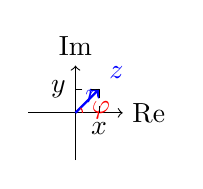
\begin{tikzpicture}[scale=0.3]
        % Coordinate axes
        \draw[->] (-2,0) -- (2,0) node[right] {Re};
        \draw[->] (0,-2) -- (0,2) node[above] {Im};
        
        % Example point and vector
        \draw[thick,blue,->] (0,0) -- (1,1) node[above right] {$z$};
        
        % Angle and labels
        \draw[red] (0.3,0) arc (0:45:0.3) node[midway,right] {$\varphi$};
        
        % Components
        \draw[dashed] (1,1) -- (1,0) node[below] {$x$};
        \draw[dashed] (1,1) -- (0,1) node[left] {$y$};
        
        % Radius
        \node[blue] at (0.7,0.7) {$r$};
    \end{tikzpicture}
\end{minipage}
\end{definition}


\begin{concept}{Darstellungsformen}
\begin{itemize}
    \item Normalform: $z = x + iy$
    \item Trigonometrische Form: $z = r(\cos\varphi + i\sin\varphi)$
    \item Exponentialform: $z = re^{i\varphi}$
\end{itemize}
\end{concept}

\begin{KR}{Umrechnung zwischen Darstellungsformen komplexer Zahlen}
\paragraph{Von Normalform in trigonometrische Form/Exponentialform}
\begin{enumerate}
   \item Berechne Betrag $r = \sqrt{x^2 + y^2}$
   \item Berechne Winkel mit einer der Formeln: 
   \begin{itemize}
       \item $\varphi = \arctan(\frac{y}{x})$ falls $x > 0$
       \item $\varphi = \arctan(\frac{y}{x}) + \pi$ falls $x < 0$
       \item $\varphi = \frac{\pi}{2}$ falls $x = 0, y > 0$
       \item $\varphi = -\frac{\pi}{2}$ falls $x = 0, y < 0$
       \item $\varphi$ unbestimmt falls $x = y = 0$
   \end{itemize}
   \item Trigonometrische Form: $z = r(\cos\varphi + i\sin\varphi)$
   \item Exponentialform: $z = re^{i\varphi}$
\end{enumerate}

\paragraph{Von trigonometrischer Form in Normalform}
\begin{enumerate}
   \item Realteil: $x = r\cos\varphi$
   \item Imaginärteil: $y = r\sin\varphi$
   \item Normalform: $z = x + iy$
\end{enumerate}

\paragraph{Von Exponentialform in Normalform/trigonometrische Form}
\begin{enumerate}
   \item Trigonometrische Form durch Euler-Formel:\\
   $re^{i\varphi} = r(\cos\varphi + i\sin\varphi)$
   \item Dann wie oben in Normalform umrechnen
\end{enumerate}

\paragraph{Wichtige Hinweise:}
\begin{itemize}
   \item Achten Sie auf das korrekte Quadranten beim Winkel
   \item Winkelfunktionen im Bogenmaß verwenden
   \item Bei Umrechnung in Normalform Euler-Formel nutzen
   \item Vorzeichen bei Exponentialform beachten
\end{itemize}
\end{KR}

\begin{KR}{Komplexe Zahlen umrechnen}
\begin{enumerate}
    \item Normalform $\leftrightarrow$ Polarform:
    \begin{itemize}
        \item Betrag: $r = \sqrt{x^2 + y^2}$
        \item Winkel: $\varphi = \arctan(\frac{y}{x})$ (Quadrant beachten!)
        \item Normalform: $z = x + iy$
        \item Polarform: $z = r(\cos\varphi + i\sin\varphi) = re^{i\varphi}$
    \end{itemize}
    
    \item Rechenoperationen:
    \begin{itemize}
        \item Addition: $(x_1 + iy_1) + (x_2 + iy_2) = (x_1+x_2) + i(y_1+y_2)$
        \item Multiplikation: $r_1r_2e^{i(\varphi_1 + \varphi_2)}$
        \item Division: $\frac{r_1}{r_2}e^{i(\varphi_1 - \varphi_2)}$
        \item n-te Potenz: $r^ne^{in\varphi}$
    \end{itemize}
\end{enumerate}
\end{KR}

\begin{example2}{Komplexe Operationen}
Gegeben $z_1 = 1+i$ und $z_2 = 2-i$:

\paragraph{Umrechnung in Polarform:}
\begin{itemize}
    \item $z_1: r_1 = \sqrt{2}$, $\varphi_1 = \frac{\pi}{4}$
    \item $z_2: r_2 = \sqrt{5}$, $\varphi_2 = -\arctan(\frac{1}{2})$
\end{itemize}

\paragraph{Berechnungen:}
\begin{itemize}
    \item $z_1 \cdot z_2 = (2-i)(1+i) = (2+1) + i(2-1) = 3+i$
    \item $z_1^3 = (\sqrt{2})^3(\cos(\frac{3\pi}{4}) + i\sin(\frac{3\pi}{4}))$
\end{itemize}
\end{example2}

\begin{theorem}{Rechenoperationen mit komplexen Zahlen}\\
Für $z_1 = x_1 + iy_1$ und $z_2 = x_2 + iy_2$ gilt:
\vspace{1mm}\\
\begin{minipage}[t]{0.45\textwidth}
    \textbf{Addition:}\\
    $z_1 + z_2 = (x_1 + x_2) + i(y_1 + y_2)$
\end{minipage}
\hspace{3mm}
\begin{minipage}[t]{0.45\textwidth}
    \textbf{Subtraktion:}\\
    $z_1 - z_2 = (x_1 - x_2) + i(y_1 - y_2)$
\end{minipage}

\begin{minipage}{0.28\textwidth}
    \textbf{Multiplikation:}
\end{minipage}
\begin{minipage}{0.68\textwidth}
    \begin{align*}
        z_1 \cdot z_2 &= (x_1x_2 - y_1y_2) + i(x_1y_2 + x_2y_1)\\
        &= r_1r_2e^{i(\varphi_1 + \varphi_2)} \text{ (in Exponentialform)}
    \end{align*}
\end{minipage}



\textbf{Division:}
\begin{align*}
    \frac{z_1}{z_2} &= \frac{z_1 \cdot z_2^*}{z_2 \cdot z_2^*} = \frac{(x_1x_2 + y_1y_2) + i(y_1x_2 - x_1y_2)}{x_2^2 + y_2^2}\\
    &= \frac{r_1}{r_2}e^{i(\varphi_1 - \varphi_2)} \text{ (in Exponentialform)}
\end{align*}
\end{theorem}

\begin{theorem}{Potenzen und Wurzeln}\\
Für eine komplexe Zahl in Exponentialform $z = re^{i\varphi}$ gilt:
\begin{itemize}
    \item n-te Potenz: $z^n = r^ne^{in\varphi} = r^n(\cos(n\varphi) + i\sin(n\varphi))$
    \item n-te Wurzel: $z_k = \sqrt[n]{r}e^{i\frac{\varphi + 2\pi k}{n}}$, $k = 0,1,\ldots,n-1$
\end{itemize}
\end{theorem}


\section{Eigenwerte und Eigenvektoren}

\begin{definition}{Eigenwerte und Eigenvektoren}\\
Für eine Matrix $A \in \mathbb{R}^{n\times n}$ heißt $\lambda \in \mathbb{C}$ Eigenwert von $A$, wenn es einen Vektor $x \in \mathbb{C}^n \backslash \{0\}$ gibt mit:
\vspace{-2mm}\\
$$Ax = \lambda x$$
Der Vektor $x$ heißt dann Eigenvektor zum Eigenwert $\lambda$.
\end{definition}

\begin{concept}{Bestimmung von Eigenwerten}\\
Ein Skalar $\lambda$ ist genau dann Eigenwert von $A$, wenn gilt:
\vspace{-2mm}\\
$$\det(A - \lambda I_n) = 0$$
Diese Gleichung heißt charakteristische Gleichung. Das zugehörige Polynom
\vspace{-2mm}
$$p(\lambda) = \det(A - \lambda I_n)$$
ist das charakteristische Polynom von $A$.
\end{concept}

\begin{theorem}{Eigenschaften von Eigenwerten}
Für eine Matrix $A \in \mathbb{R}^{n\times n}$ gilt:
$$\det(A) = \prod_{i=1}^n \lambda_i \text{ (Produkt der Eigenwerte)}$$
$$\operatorname{tr}(A) = \sum_{i=1}^n \lambda_i \text{ (Summe der Eigenwerte)}$$
\begin{itemize}
    \item Bei Dreiecksmatrix sind die Diagonalelemente die Eigenwerte
    \item Ist $\lambda$ Eigenwert von $A$, so ist $\frac{1}{\lambda}$ Eigenwert von $A^{-1}$
\end{itemize}
\end{theorem}

\begin{concept}{Vielfachheiten}
Für einen Eigenwert $\lambda$ unterscheidet man:
\begin{itemize}
    \item Algebraische Vielfachheit: \\Vielfachheit als Nullstelle des charakteristischen Polynoms
    \item Geometrische Vielfachheit: \\Dimension des Eigenraums $= n - \operatorname{rg}(A-\lambda I_n)$
\end{itemize}
Die geometrische Vielfachheit ist stets kleiner oder gleich der algebraischen Vielfachheit.
\end{concept}

\begin{KR}{Bestimmung von Eigenwerten und Eigenvektoren}
\paragraph{Vorbereitung}
\begin{itemize}
    \item Matrix $A \in \mathbb{R}^{n \times n}$ aufschreiben
    \item Charakteristische Matrix $(A - \lambda I)$ aufstellen
\end{itemize}

\paragraph{Eigenwerte bestimmen}
\begin{enumerate}
    \item Charakteristisches Polynom aufstellen:
    \begin{itemize}
        \item Bei $2 \times 2$ Matrizen direkt: $\det(A - \lambda I)$
        \item Bei $3 \times 3$ Matrizen: Entwicklung nach einer Zeile/Spalte
        \item Bei größeren Matrizen: Spezielle Eigenschaften nutzen
              (z.B. Dreiecksform, Symmetrie)
    \end{itemize}
    
    \item Polynom vereinfachen und auf Nullform bringen:
    \begin{itemize}
        \item Ausmultiplizieren
        \item Zusammenfassen nach Potenzen von $\lambda$
        \item Form: $p(\lambda) = (-1)^n\lambda^n + a_{n-1}\lambda^{n-1} + \cdots + a_1\lambda + a_0$
    \end{itemize}

    \item Nullstellen bestimmen:
    \begin{itemize}
        \item Bei quadratischer Gleichung: Mitternachtsformel
        \item Bei Grad 3: Substitution oder Cardanische Formeln
        \item Bei höherem Grad: Numerische Verfahren
    \end{itemize}
\end{enumerate}

\paragraph{Eigenvektoren bestimmen}
\begin{enumerate}
    \item Für jeden Eigenwert $\lambda_i$:
    \begin{itemize}
        \item Matrix $(A - \lambda_i I)$ aufstellen
        \item Homogenes LGS $(A - \lambda_i I)x = 0$ lösen
        \item Lösungsvektor normieren falls gewünscht
    \end{itemize}

    \item Bei mehrfachen Eigenwerten:
    \begin{itemize}
        \item Basis des Eigenraums bestimmen
        \item Linear unabhängige Eigenvektoren finden
    \end{itemize}
\end{enumerate}

\paragraph{Kontrolle}
\begin{itemize}
    \item Für jeden Eigenvektor $x_i$ prüfen: $Ax_i = \lambda_i x_i$
    \item Bei $2 \times 2$ Matrix: $\lambda_1 + \lambda_2 = \operatorname{tr}(A)$ und $\lambda_1 \cdot \lambda_2 = \det(A)$
    \item Bei $3 \times 3$ Matrix zusätzlich: $\sum \lambda_i = \operatorname{tr}(A)$ und $\prod \lambda_i = \det(A)$
    \item Bei reellen Matrizen: Komplexe Eigenwerte treten in konjugierten Paaren auf
\end{itemize}

\paragraph{Spezialfälle beachten}
\begin{itemize}
    \item Bei Dreiecksmatrizen: Eigenwerte sind die Diagonalelemente
    \item Bei symmetrischen Matrizen: Alle Eigenwerte sind reell
    \item Bei orthogonalen Matrizen: $|\lambda_i| = 1$ für alle Eigenwerte
    \item Bei nilpotenten Matrizen: Alle Eigenwerte sind 0
\end{itemize}
\end{KR}

\begin{example2}{Eigenwertberechnung}
Gegeben ist die Matrix
$A = \begin{psmallmatrix} 
2 & 1 & 0 \\
1 & 2 & 1 \\
0 & 1 & 2
\end{psmallmatrix}$

1. Charakteristisches Polynom aufstellen:
   $$\det(A - \lambda I) = \begin{vsmallmatrix} 
   2-\lambda & 1 & 0 \\
   1 & 2-\lambda & 1 \\
   0 & 1 & 2-\lambda
   \end{vsmallmatrix}$$
   
2. Entwicklung nach 1. Zeile:
   $$p(\lambda) = (2-\lambda)\begin{vsmallmatrix}
   2-\lambda & 1 \\
   1 & 2-\lambda
   \end{vsmallmatrix} - 1\begin{vsmallmatrix}
   1 & 1 \\
   1 & 2-\lambda
   \end{vsmallmatrix}$$
   
3. Ausrechnen:
   $$p(\lambda) = (2-\lambda)((2-\lambda)^2 - 1) - ((2-\lambda) - 1)
   = -\lambda^3 + 6\lambda^2 - 11\lambda + 6$$
   
4. Nullstellen bestimmen:
   $\lambda_1 = 1, \lambda_2 = 2, \lambda_3 = 3$
\vspace{1mm}\\
5. Eigenvektoren bestimmen für $\lambda_1 = 1$:
   $$(A - I)x = 0 \text{ führt zu } x_1 = \begin{psmallmatrix} 1 \\ -2 \\ 1 \end{psmallmatrix}$$
\end{example2}

\begin{KR}{Eigenwerte bestimmen}
\begin{enumerate}
    \item Charakteristisches Polynom aufstellen:
    \begin{itemize}
        \item $p(\lambda) = \det(A-\lambda I)$ berechnen
        \item Auf Standardform bringen
    \end{itemize}
    
    \item Nullstellen bestimmen:
    \begin{itemize}
        \item Quadratische Formel für $n=2$
        \item Cardano-Formel für $n=3$
        \item Numerische Verfahren für $n>3$
    \end{itemize}
    
    \item Vielfachheiten bestimmen:
    \begin{itemize}
        \item Algebraische Vielfachheit: Nullstellenordnung
        \item Geometrische Vielfachheit: $n-\operatorname{rang}(A-\lambda I)$
    \end{itemize}
\end{enumerate}
\end{KR}

\begin{example2}{Charakteristisches Polynom}
Bestimmen Sie die Eigenwerte von:
$$A = \begin{pmatrix}
2 & -1 & 0 \\
-1 & 2 & -1 \\
0 & -1 & 2
\end{pmatrix}$$

\paragraph{Lösung:}
\begin{enumerate}
    \item $p(\lambda) = \det(A-\lambda I)$:
    $$\begin{vmatrix}
    2-\lambda & -1 & 0 \\
    -1 & 2-\lambda & -1 \\
    0 & -1 & 2-\lambda
    \end{vmatrix}$$
    
    \item Determinante entwickeln:
    $$p(\lambda) = (2-\lambda)^3 - 2(2-\lambda) = -\lambda^3 + 6\lambda^2 - 11\lambda + 6$$
    
    \item Nullstellen:
    $$\lambda_1 = 1, \lambda_2 = 2, \lambda_3 = 3$$
\end{enumerate}
\end{example2}

\begin{KR}{Eigenvektoren bestimmen}
\begin{enumerate}
    \item Für jeden Eigenwert $\lambda$:
    \begin{itemize}
        \item $(A-\lambda I)x = 0$ aufstellen
        \item Homogenes LGS lösen
        \item Lösungsvektor normieren
    \end{itemize}
    
    \item Bei mehrfachen Eigenwerten:
    \begin{itemize}
        \item Geometrische Vielfachheit bestimmen
        \item Basis des Eigenraums finden
    \end{itemize}
    
    \item Kontrolle:
    \begin{itemize}
        \item $Ax = \lambda x$ überprüfen
        \item Orthogonalität bei symmetrischen Matrizen
        \item Linear unabhängig?
    \end{itemize}
\end{enumerate}
\end{KR}

\begin{example2}{Eigenvektoren}
Bestimmen Sie die Eigenvektoren zum Eigenwert $\lambda=2$ der Matrix:
$$A = \begin{pmatrix}
2 & 1 & 0 \\
0 & 2 & 0 \\
0 & -1 & 2
\end{pmatrix}$$

\paragraph{Lösung:}
\begin{enumerate}
    \item $(A-2I)x = 0$:
    $$\begin{pmatrix}
    0 & 1 & 0 \\
    0 & 0 & 0 \\
    0 & -1 & 0
    \end{pmatrix} \begin{pmatrix}
    x_1 \\ x_2 \\ x_3
    \end{pmatrix} = \begin{pmatrix}
    0 \\ 0 \\ 0
    \end{pmatrix}$$
    
    \item Homogenes System lösen:
    \begin{itemize}
        \item $x_2 = 0$ (aus 1. Zeile)
        \item $x_1, x_3$ frei wählbar
    \end{itemize}
    
    \item Basis des Eigenraums:
    $$v_1 = \begin{pmatrix} 1 \\ 0 \\ 0 \end{pmatrix}, 
    v_2 = \begin{pmatrix} 0 \\ 0 \\ 1 \end{pmatrix}$$
\end{enumerate}
\end{example2}

\subsubsection{Numerische Berechnung von Eigenwerten}

\begin{concept}{Ähnliche Matrizen}\\
Zwei Matrizen $A,B \in \mathbb{R}^{n\times n}$ heißen ähnlich, wenn es eine reguläre Matrix $T$ gibt mit:
$$B = T^{-1}AT$$

Eine Matrix $A$ heißt diagonalisierbar, wenn sie ähnlich zu einer Diagonalmatrix $D$ ist:
$$D = T^{-1}AT$$
\end{concept}

\begin{theorem}{Eigenschaften ähnlicher Matrizen}\\
Für ähnliche Matrizen $A$ und $B = T^{-1}AT$ gilt:
\begin{enumerate}
    \item $A$ und $B$ haben dieselben Eigenwerte mit gleichen algebraischen Vielfachheiten
    \item Ist $x$ Eigenvektor von $B$ zum Eigenwert $\lambda$, so ist $Tx$ Eigenvektor von $A$ zum Eigenwert $\lambda$
    \item Bei Diagonalisierbarkeit:
    \begin{itemize}
        \item Die Diagonalelemente von $D$ sind die Eigenwerte von $A$
        \item Die Spalten von $T$ sind die Eigenvektoren von $A$
    \end{itemize}
\end{enumerate}
\end{theorem}

\begin{definition}{Spektralradius}
Der Spektralradius einer Matrix $A$ ist definiert als:
$$\rho(A) = \max\{|\lambda| \mid \lambda \text{ ist Eigenwert von } A\}$$
Er gibt den Betrag des betragsmäßig größten Eigenwerts an.
\end{definition}

\subsubsection{Von-Mises-Iteration}

\begin{concept}{Von-Mises-Iteration (Vektoriteration)}\\
Für eine diagonalisierbare Matrix $A$ mit Eigenwerten $|\lambda_1| > |\lambda_2| \geq \cdots \geq |\lambda_n|$ konvergiert die Folge:
$$v^{(k+1)} = \frac{Av^{(k)}}{\|Av^{(k)}\|_2}, \quad
\lambda^{(k+1)} = \frac{(v^{(k)})^TAv^{(k)}}{(v^{(k)})^Tv^{(k)}}$$
gegen einen Eigenvektor $v$ zum betragsmäßig größten Eigenwert $\lambda_1$.
\end{concept}

\begin{KR}{Von-Mises-Iteration / Vektoriteration}
\paragraph{Algorithmus}
\begin{enumerate}
    \item Startvektor $v^{(0)}$ wählen:
    \begin{itemize}
        \item Zufälligen Vektor oder $(1,\ldots,1)^T$ wählen
        \item Auf Länge 1 normieren: $\|v^{(0)}\|_2 = 1$
    \end{itemize}

    \item Für $k = 0,1,2,\ldots$ bis zur Konvergenz:
    \begin{itemize}
        \item Iterationsvektor berechnen: $w^{(k)} = Av^{(k)}$
        \item Normieren: $v^{(k+1)} = \frac{w^{(k)}}{\|w^{(k)}\|_2}$
        \item Eigenwertapproximation (Rayleigh-Quotient):
              $$\lambda^{(k+1)} = \frac{(v^{(k)})^TAv^{(k)}}{(v^{(k)})^Tv^{(k)}}$$
    \end{itemize}

    \item Abbruchkriterien prüfen:
    \begin{itemize}
        \item Änderung des Eigenvektors: $\|v^{(k+1)} - v^{(k)}\| < \varepsilon$
        \item Änderung des Eigenwertes: $|\lambda^{(k+1)} - \lambda^{(k)}| < \varepsilon$
        \item Maximale Iterationszahl erreicht
    \end{itemize}
\end{enumerate}

\paragraph{Verifikation}
\begin{itemize}
    \item Prüfen ob $Av^{(k)} \approx \lambda^{(k)}v^{(k)}$
    \item Residuum berechnen: $\|Av^{(k)} - \lambda^{(k)}v^{(k)}\|$
    \item Orthogonalität zu anderen Eigenvektoren prüfen
\end{itemize}
\end{KR}

\begin{example2}{Von-Mises-Iteration}
Gegeben sei die Matrix
$A = \begin{psmallmatrix} 
4 & -1 & 1 \\
-1 & 3 & -2 \\
1 & -2 & 3
\end{psmallmatrix}$

Mit Startvektor $v^{(0)} = \frac{1}{\sqrt{3}}(1,1,1)^T$:

\begin{enumerate}
    \item Erste Iteration:
    \begin{itemize}
        \item $w^{(0)} = Av^{(0)} = \frac{1}{\sqrt{3}}(4,0,2)^T$
        \item $v^{(1)} = \frac{w^{(0)}}{\|w^{(0)}\|} = \frac{1}{\sqrt{20}}(4,0,2)^T$
        \item $\lambda^{(1)} = (v^{(0)})^TAv^{(0)} = 3.33$
    \end{itemize}

    \item Zweite Iteration:
    \begin{itemize}
        \item $w^{(1)} = Av^{(1)} = \frac{1}{\sqrt{20}}(18,-2,8)^T$
        \item $v^{(2)} = \frac{w^{(1)}}{\|w^{(1)}\|} = \frac{1}{\sqrt{388}}(18,-2,8)^T$
        \item $\lambda^{(2)} = 5.12$
    \end{itemize}

Konvergenz gegen $\lambda_1 \approx 5.17$ und $v = (0.89, -0.10, 0.39)^T$
\end{enumerate}
\end{example2}

\begin{KR}{Vektoriteration durchführen}
\begin{enumerate}
    \item Voraussetzungen prüfen:
    \begin{itemize}
        \item Matrix diagonalisierbar
        \item $|\lambda_1| > |\lambda_2|$
    \end{itemize}
    
    \item Iteration:
    \begin{itemize}
        \item $w^{(k)} = Av^{(k)}$
        \item $v^{(k+1)} = \frac{w^{(k)}}{\|w^{(k)}\|}$
        \item $\lambda^{(k+1)} = \frac{(v^{(k)})^TAv^{(k)}}{(v^{(k)})^Tv^{(k)}}$
    \end{itemize}
    
    \item Konvergenz:
    \begin{itemize}
        \item $v^{(k)} \to$ Eigenvektor zu $|\lambda_1|$
        \item $\lambda^{(k)} \to |\lambda_1|$
    \end{itemize}
\end{enumerate}
\end{KR}

\begin{example2}{Von-Mises-Iteration}
Bestimmen Sie den betragsmäßig größten Eigenwert von:
$$A = \begin{pmatrix}
3 & 1 \\
1 & 3
\end{pmatrix}$$

\paragraph{Lösung:}
\begin{enumerate}
    \item Start mit $v^{(0)} = \frac{1}{\sqrt{2}}\begin{pmatrix} 1 \\ 1 \end{pmatrix}$
    
    \item Erste Iteration:
    \begin{itemize}
        \item $w^{(0)} = \begin{pmatrix} 4 \\ 4 \end{pmatrix}$
        \item $v^{(1)} = \frac{1}{\sqrt{2}}\begin{pmatrix} 1 \\ 1 \end{pmatrix}$
        \item $\lambda^{(1)} = 4$
    \end{itemize}
    
    \item Ergebnis:
    \begin{itemize}
        \item Eigenvektor bereits gefunden
        \item Eigenwert $\lambda = 4$ ist korrekt
    \end{itemize}
\end{enumerate}
\end{example2}

\subsubsection{QR-Verfahren}

\begin{concept}{QR-Verfahren}\\
Das QR-Verfahren transformiert die Matrix $A$ iterativ in eine obere Dreiecksmatrix, deren Diagonalelemente die Eigenwerte sind:
\begin{enumerate}
    \item Initialisierung: $A_0 := A$, $P_0 := I_n$
    \item Für $i = 0,1,2,\ldots$:
    \begin{itemize}
        \item QR-Zerlegung: $A_i = Q_iR_i$
        \item Neue Matrix: $A_{i+1} = R_iQ_i$
        \item Update: $P_{i+1} = P_iQ_i$
    \end{itemize}
\end{enumerate}
\end{concept}

\begin{KR}{QR-Verfahren}
\paragraph{Voraussetzungen}
\begin{itemize}
    \item Matrix $A \in \mathbb{R}^{n \times n}$
    \item Eigenwerte sollten verschiedene Beträge haben für gute Konvergenz
\end{itemize}

\paragraph{Algorithmus}
\begin{enumerate}
    \item Initialisierung:
    \begin{itemize}
        \item $A_0 := A$
        \item $Q_0 := I_n$
    \end{itemize}

    \item Für $k = 0,1,2,\ldots$ bis zur Konvergenz:
    \begin{itemize}
        \item QR-Zerlegung von $A_k$ berechnen: $A_k = Q_kR_k$
        \item Neue Matrix berechnen: $A_{k+1} = R_kQ_k$
        \item Transformationsmatrix aktualisieren: $P_{k+1} = P_kQ_k$
    \end{itemize}

    \item Abbruchkriterien prüfen:
    \begin{itemize}
        \item Subdiagonalelemente nahe Null: $|a_{i+1,i}| < \varepsilon$
        \item Änderung der Diagonalelemente klein
        \item Maximale Iterationszahl erreicht
    \end{itemize}
\end{enumerate}

\paragraph{Auswertung}
\begin{itemize}
    \item Eigenwerte: Diagonalelemente von $A_k$
    \item Eigenvektoren: Spalten der Matrix $P_k$
    \item Bei $2\times2$-Blöcken: Komplexe Eigenwertpaare
\end{itemize}
\end{KR}

\begin{example2}{QR-Verfahren}
Gegeben sei die Matrix
$A = \begin{psmallmatrix} 
1 & 2 & 0 \\
2 & 1 & 1 \\
0 & 1 & 1
\end{psmallmatrix}$

\begin{enumerate}
    \item Erste Iteration:
    \begin{itemize}
        \item QR-Zerlegung:
        $Q_1 = \begin{psmallmatrix} 
        0.45 & 0.89 & 0 \\
        0.89 & -0.45 & 0 \\
        0 & 0 & 1
        \end{psmallmatrix}$,
        $R_1 = \begin{psmallmatrix}
        2.24 & 2.24 & 0.45 \\
        0 & -1 & 0.89 \\
        0 & 0 & 1
        \end{psmallmatrix}$
        \item $A_1 = R_1Q_1 = \begin{psmallmatrix}
        2.24 & 0.45 & 0.45 \\
        0.45 & 0.38 & 0.89 \\
        0.45 & 0.89 & 1
        \end{psmallmatrix}$
    \end{itemize}

    \item Nach Konvergenz:
    $A_k \approx \begin{psmallmatrix}
    3 & * & * \\
    0 & 0 & * \\
    0 & 0 & 0
    \end{psmallmatrix}$

    Eigenwerte sind also $\lambda_1 = 3, \lambda_2 = 0, \lambda_3 = 0$
\end{enumerate}
\end{example2}

\begin{KR}{QR-Algorithmus anwenden}
\begin{enumerate}
    \item Initialisierung:
    \begin{itemize}
        \item $A_0 := A$
        \item $Q_0 := I_n$
    \end{itemize}
    
    \item Iteration:
    \begin{itemize}
        \item QR-Zerlegung: $A_k = Q_kR_k$
        \item Neue Matrix: $A_{k+1} = R_kQ_k$
        \item Update: $P_{k+1} = P_kQ_k$
    \end{itemize}
    
    \item Abbruch wenn:
    \begin{itemize}
        \item Subdiagonalelemente klein
        \item Diagonalelemente konvergieren
        \item Maximale Iterationen erreicht
    \end{itemize}
\end{enumerate}
\end{KR}

\begin{example2}{QR-Iteration}
Führen Sie eine QR-Iteration durch für:
$$A = \begin{pmatrix}
1 & 1 \\
1 & 0
\end{pmatrix}$$

\paragraph{Lösung:}
\begin{enumerate}
    \item QR-Zerlegung von $A$:
    $$Q_1 = \frac{1}{\sqrt{2}}\begin{pmatrix}
    1 & -1 \\
    1 & 1
    \end{pmatrix}, 
    R_1 = \frac{1}{\sqrt{2}}\begin{pmatrix}
    \sqrt{2} & 1 \\
    0 & -1
    \end{pmatrix}$$
    
    \item Neue Matrix:
    $$A_1 = R_1Q_1 = \begin{pmatrix}
    1.5 & 0.5 \\
    0.5 & -0.5
    \end{pmatrix}$$
    
    \item Konvergenz nach mehreren Iterationen gegen:
    $$A_\infty \approx \begin{pmatrix}
    \phi & 0 \\
    0 & -\phi^{-1}
    \end{pmatrix}$$
    mit $\phi = \frac{1+\sqrt{5}}{2}$
\end{enumerate}
\end{example2}





\begin{KR}{Numerische Aspekte}
\begin{enumerate}
    \item Wahl des Startpunkts:
    \begin{itemize}
        \item Von-Mises: zufälliger normierter Vektor
        \item Inverse Iteration: Näherung für $\mu$ wichtig
        \item QR: Matrix vorher auf Hessenberg-Form
    \end{itemize}
    
    \item Konvergenzprüfung:
    \begin{itemize}
        \item Residuum $\|Ax^{(k)} - \lambda^{(k)}x^{(k)}\|$
        \item Änderung in aufeinanderfolgenden Iterationen
        \item Subdiagonalelemente bei QR
    \end{itemize}
    
    \item Spezialfälle:
    \begin{itemize}
        \item Mehrfache Eigenwerte
        \item Komplexe Eigenwerte/vektoren
        \item Schlecht konditionierte Matrizen
    \end{itemize}
\end{enumerate}
\end{KR}


\subsection{Eigenwerte und Eigenvektoren}

\begin{definition}{Eigenwerte und Eigenvektoren}
Für eine Matrix $A \in \mathbb{R}^{n \times n}$ ist $\lambda \in \mathbb{C}$ ein Eigenwert und $x \in \mathbb{C}^n \setminus \{0\}$ ein zugehöriger Eigenvektor, wenn gilt:
$$Ax = \lambda x$$
\end{definition}

\begin{concept}{Spektralradius}
Der Spektralradius $\rho(A)$ einer Matrix $A$ ist der betragsmäßig größte Eigenwert:
$$\rho(A) = \max\{|\lambda| : \lambda \text{ ist Eigenwert von } A\}$$
Der Spektralradius spielt eine wichtige Rolle bei der Konvergenz iterativer Verfahren.
\end{concept}

\begin{KR}{Bestimmung von Eigenwerten und Eigenvektoren}
\begin{enumerate}
    \item Eigenwerte bestimmen:
    \begin{itemize}
        \item Charakteristisches Polynom aufstellen: $p(\lambda) = \det(A-\lambda I)$
        \item Nullstellen von $p(\lambda)$ finden
    \end{itemize}
    
    \item Für jeden Eigenwert $\lambda$:
    \begin{itemize}
        \item Löse $(A-\lambda I)x = 0$ 
        \item Bestimme Basisvektoren des Eigenraums
        \item Normiere die Eigenvektoren falls gewünscht
    \end{itemize}
    
    \item Bei QR-Verfahren:
    \begin{itemize}
        \item QR-Zerlegung iterativ durchführen
        \item Diagonalelemente konvergieren gegen Eigenwerte
        \item Produkt der Q-Matrizen ergibt Eigenvektoren
    \end{itemize}
\end{enumerate}
\end{KR}

\begin{example2}{Eigenwerte und Eigenvektoren}
Bestimmen Sie Eigenwerte und -vektoren von:
$$A = \begin{pmatrix}
2 & -1 \\
-1 & 2
\end{pmatrix}$$

\paragraph{Lösung:}
\begin{enumerate}
    \item Charakteristisches Polynom:
    $$\det(A-\lambda I) = \begin{vmatrix} 
    2-\lambda & -1 \\
    -1 & 2-\lambda
    \end{vmatrix} = (2-\lambda)^2 - 1 = 0$$
    
    \item Eigenwerte: $\lambda_1 = 3$, $\lambda_2 = 1$
    
    \item Eigenvektoren für $\lambda_1 = 3$:
    $$(A-3I)x = \begin{pmatrix}
    -1 & -1 \\
    -1 & -1
    \end{pmatrix}x = 0 \Rightarrow x_1 = \begin{pmatrix}
    1 \\
    1
    \end{pmatrix}$$
    
    \item Eigenvektoren für $\lambda_2 = 1$:
    $$(A-I)x = \begin{pmatrix}
    1 & -1 \\
    -1 & 1
    \end{pmatrix}x = 0 \Rightarrow x_2 = \begin{pmatrix}
    1 \\
    -1
    \end{pmatrix}$$
\end{enumerate}
\end{example2}

\begin{KR}{Numerische Eigenwertberechnung mit QR-Verfahren}
\begin{enumerate}
    \item Vorbereitung:
    \begin{itemize}
        \item Matrix $A_0 := A$ setzen
        \item Maximale Iterationszahl und Toleranz festlegen
    \end{itemize}
    
    \item QR-Iteration:
    \begin{itemize}
        \item QR-Zerlegung: $A_k = Q_kR_k$
        \item Neue Matrix: $A_{k+1} = R_kQ_k$
        \item Eigenvektormatrix: $V_{k+1} = V_kQ_k$
    \end{itemize}
    
    \item Konvergenzprüfung:
    \begin{itemize}
        \item Nebendiagonalelemente nahe Null?
        \item Änderung der Diagonalelemente klein genug?
        \item Maximale Iterationen erreicht?
    \end{itemize}
\end{enumerate}
\end{KR}

\begin{example2}{QR-Verfahren}
Bestimmen Sie die Eigenwerte der Matrix mit dem QR-Verfahren:
$$A = \begin{pmatrix}
1 & -1 \\
4 & 3
\end{pmatrix}$$

\paragraph{Erste Iteration:}
\begin{enumerate}
    \item QR-Zerlegung von $A_0$:
    $$Q_1 = \begin{pmatrix}
    0.2425 & -0.9701 \\
    0.9701 & 0.2425
    \end{pmatrix}, 
    R_1 = \begin{pmatrix}
    4.1231 & 2.6656 \\
    0 & -0.3656
    \end{pmatrix}$$
    
    \item Neue Matrix $A_1 = R_1Q_1$:
    $$A_1 = \begin{pmatrix}
    3.8 & -0.9 \\
    0.9 & 0.2
    \end{pmatrix}$$
\end{enumerate}

Nach weiteren Iterationen konvergiert $A_k$ gegen eine obere Dreiecksmatrix,
deren Diagonalelemente die Eigenwerte sind: $\lambda_1 \approx 4$, $\lambda_2 \approx 0$.
\end{example2}

\subsubsection{Inverse Iteration}

\begin{concept}{Inverse Iteration}
Die inverse Iteration berechnet einen Eigenvektor zu einem bekannten oder geschätzten Eigenwert $\mu$ durch:
$$v^{(k+1)} = \frac{(A-\mu I)^{-1}v^{(k)}}{\|(A-\mu I)^{-1}v^{(k)}\|_2}$$
Konvergiert typischerweise gegen den Eigenvektor zum betragsmäßig kleinsten Eigenwert $\lambda_i - \mu$.
\end{concept}

\begin{KR}{Inverse Iteration anwenden}
\begin{enumerate}
    \item Vorbereitung:
    \begin{itemize}
        \item Näherungswert $\mu$ für Eigenwert wählen
        \item Zufälligen Startvektor $v^{(0)}$ normieren 
        \item LR-Zerlegung von $(A-\mu I)$ berechnen
    \end{itemize}
    
    \item Iteration durchführen:
    \begin{itemize}
        \item LR-System $(A-\mu I)w^{(k)} = v^{(k)}$ lösen
        \item Neuen Vektor normieren: $v^{(k+1)} = \frac{w^{(k)}}{\|w^{(k)}\|_2}$
        \item Rayleigh-Quotient berechnen für Eigenwert
    \end{itemize}
    
    \item Abbruch wenn:
    \begin{itemize}
        \item Residuum $\|(A-\lambda^{(k)}I)v^{(k)}\| < \epsilon$
        \item Maximale Iterationszahl erreicht
    \end{itemize}
\end{enumerate}
\end{KR}

\begin{example2}{Inverse Iteration}
Bestimmen Sie einen Eigenvektor zum Eigenwert $\lambda \approx 2$ der Matrix:
$$A = \begin{pmatrix}
2.1 & -0.1 & 0.1 \\
-0.1 & 2.0 & 0.2 \\
0.1 & 0.2 & 1.9
\end{pmatrix}$$

\paragraph{Lösung:}
\begin{enumerate}
    \item $\mu = 2.0$ als Näherung wählen
    \item Startvektor $v^{(0)} = \frac{1}{\sqrt{3}}(1,1,1)^T$
    \item Erste Iteration:
    \begin{itemize}
        \item $(A-2I)w^{(0)} = v^{(0)}$ lösen
        \item $v^{(1)} = \frac{w^{(0)}}{\|w^{(0)}\|} \approx (0.61, 0.63, 0.48)^T$
        \item $\lambda^{(1)} \approx 2.01$
    \end{itemize}
\end{enumerate}
\end{example2}

\begin{KR}{Vergleich der Eigenwertverfahren}
\begin{enumerate}
    \item Von-Mises Iteration:
    \begin{itemize}
        \item Findet betragsmäßig größten Eigenwert
        \item Einfach zu implementieren
        \item Langsame lineare Konvergenz
    \end{itemize}
    
    \item Inverse Iteration:
    \begin{itemize}
        \item Braucht Näherung für Eigenwert
        \item Schnelle Konvergenz
        \item LR-Zerlegung pro Schritt nötig
    \end{itemize}
    
    \item QR-Verfahren:
    \begin{itemize}
        \item Berechnet alle Eigenwerte 
        \item Kubischer Aufwand pro Iteration
        \item Globale und stabile Konvergenz
    \end{itemize}
\end{enumerate}
\end{KR}

\begin{example2}{Numerischer Vergleich}
\small
Matrix $A = \begin{pmatrix} 4 & -1 \\ 1 & 3 \end{pmatrix}$ mit $\lambda_1 = 5, \lambda_2 = 2$
\begin{center}
\begin{tabular}{l|c|c|c}
Verfahren & Iterationen & Genauigkeit & Zeit\\
\hline
Von-Mises & 23 & $10^{-8}$ & 1.0\\
Inverse Iteration & 6 & $10^{-8}$ & 1.5\\  
QR & 8 & $10^{-12}$ & 2.3\\
\end{tabular}
\end{center}

\paragraph{Beobachtungen:}
\begin{itemize}
    \item Von-Mises braucht viele Iterationen
    \item Inverse Iteration konvergiert schnell
    \item QR liefert höchste Genauigkeit
\end{itemize}
\end{example2}

\begin{KR}{Typische Prüfungsaufgaben}
\begin{enumerate}
    \item Theorieaufgaben:
    \begin{itemize}
        \item Eigenschaften von Eigenwerten beweisen
        \item Konvergenzverhalten analysieren
        \item Spezialfälle untersuchen
    \end{itemize}
    
    \item Rechenaufgaben:
    \begin{itemize}
        \item Charakteristisches Polynom aufstellen
        \item Eigenwerte/vektoren bestimmen
        \item 2-3 Iterationsschritte durchführen
    \end{itemize}
    
    \item Implementierungsaufgaben:
    \begin{itemize}
        \item Verfahren in Python implementieren
        \item Konvergenzverhalten visualisieren
        \item Verfahren vergleichen
    \end{itemize}
\end{enumerate}
\end{KR}

\subsection{Spektralradius und Anwendungen}

\begin{definition}{Spektralradius}
Der Spektralradius $\rho(A)$ einer Matrix $A \in \mathbb{R}^{n\times n}$ ist definiert als der größte Absolutbetrag ihrer Eigenwerte:
$$\rho(A) = \max\{|\lambda| \mid \lambda \text{ ist Eigenwert von } A\}$$
\end{definition}

\begin{concept}{Bedeutung des Spektralradius}
Der Spektralradius ist wichtig für:
\begin{itemize}
    \item Konvergenz von Iterationsverfahren
    \item Stabilität dynamischer Systeme 
    \item Abschätzung von Matrixnormen
    \item Konvergenz von Potenzreihen mit Matrizen
\end{itemize}
\end{concept}

\begin{theorem}{Konvergenzsatz}
Für eine Matrix $A \in \mathbb{R}^{n\times n}$ sind äquivalent:
\begin{itemize}
    \item $\rho(A) < 1$
    \item $\lim_{k\to\infty} A^k = 0$
    \item Die Neumannsche Reihe $\sum_{k=0}^\infty A^k$ konvergiert
    \item $(I-A)$ ist invertierbar mit $(I-A)^{-1} = \sum_{k=0}^\infty A^k$
\end{itemize}
\end{theorem}

\begin{KR}{Spektralradius bestimmen und anwenden}
\begin{enumerate}
    \item Berechnung:
    \begin{itemize}
        \item Eigenwerte $\lambda_i$ bestimmen
        \item Maximum der Absolutbeträge bilden
        \item Bei großen Matrizen: numerische Verfahren
    \end{itemize}
    
    \item Konvergenzanalyse:
    \begin{itemize}
        \item Bei Iterationsverfahren: $\rho(M) < 1$ prüfen
        \item Bei Matrixpotenzen: $\rho(A) < 1$ prüfen
        \item Konvergenzgeschwindigkeit $\approx |\rho(A)|^k$
    \end{itemize}
    
    \item Abschätzungen:
    \begin{itemize}
        \item $\rho(A) \leq \|A\|$ für jede Matrixnorm
        \item $\rho(AB) = \rho(BA)$ für beliebige Matrizen
        \item $\rho(A^k) = [\rho(A)]^k$ für $k \in \mathbb{N}$
    \end{itemize}
\end{enumerate}
\end{KR}

\begin{example2}{Spektralradius und Konvergenz}
Untersuchen Sie die Konvergenz des Jacobi-Verfahrens für:
$$A = \begin{pmatrix}
4 & -1 & 0 \\
-1 & 4 & -1 \\
0 & -1 & 4
\end{pmatrix}$$

\paragraph{Lösung:}
\begin{enumerate}
    \item Zerlegung $A = D + L + R$:
    $$D = \begin{pmatrix}
    4 & 0 & 0 \\
    0 & 4 & 0 \\
    0 & 0 & 4
    \end{pmatrix}, L+R = \begin{pmatrix}
    0 & -1 & 0 \\
    -1 & 0 & -1 \\
    0 & -1 & 0
    \end{pmatrix}$$
    
    \item Jacobi-Matrix $M = -D^{-1}(L+R)$:
    $$M = \begin{pmatrix}
    0 & 1/4 & 0 \\
    1/4 & 0 & 1/4 \\
    0 & 1/4 & 0
    \end{pmatrix}$$
    
    \item Eigenwerte von $M$: $\lambda_1 = 0.5$, $\lambda_2 = 0$, $\lambda_3 = -0.5$
    
    \item Spektralradius: $\rho(M) = 0.5 < 1$
    
    \item Schlussfolgerung:
    \begin{itemize}
        \item Jacobi-Verfahren konvergiert
        \item Fehler reduziert sich pro Iteration etwa um Faktor 0.5
        \item Konvergenzrate ist linear
    \end{itemize}
\end{enumerate}
\end{example2}

\begin{KR}{Anwendungen des Spektralradius}
\begin{enumerate}
    \item Iterative Verfahren:
    \begin{itemize}
        \item Jacobi: $\rho(-D^{-1}(L+R)) < 1$
        \item Gauss-Seidel: $\rho(-(D+L)^{-1}R) < 1$
        \item SOR: Optimaler Parameter $\omega$ bestimmen
    \end{itemize}
    
    \item Matrixreihen:
    \begin{itemize}
        \item Konvergenz von $\sum_{k=0}^\infty A^k$
        \item Existenz von $(I-A)^{-1}$
        \item Abschätzung der Reihensumme
    \end{itemize}
    
    \item Stabilitätsanalyse:
    \begin{itemize}
        \item Diskrete dynamische Systeme
        \item Numerische Integration
        \item Differenzenverfahren
    \end{itemize}
\end{enumerate}
\end{KR}

\begin{example2}{Matrixreihe}
Untersuchen Sie die Konvergenz der Reihe $\sum_{k=0}^\infty A^k$ für:
$$A = \begin{pmatrix}
0 & 1/2 \\
1/2 & 0
\end{pmatrix}$$

\paragraph{Lösung:}
\begin{enumerate}
    \item Eigenwerte bestimmen:
    $$\det(A-\lambda I) = \lambda^2 - \frac{1}{4} = 0 \Rightarrow \lambda_{1,2} = \pm\frac{1}{2}$$
    
    \item Spektralradius:
    $$\rho(A) = \max\{|-\frac{1}{2}|, |\frac{1}{2}|\} = \frac{1}{2} < 1$$
    
    \item Schlussfolgerungen:
    \begin{itemize}
        \item Reihe konvergiert
        \item $(I-A)$ ist invertierbar
        \item Summe ist $(I-A)^{-1}$
    \end{itemize}
\end{enumerate}
\end{example2}






	\raggedcolumns
	
	\section{Python Implementationen}

\subsubsection{Hilfsfunktionen}

\begin{examplecode}{Matrixoperationen}
\begin{lstlisting}[language=Python, style=basesmol]
def matrix_vector_mult(A, v): # Matrix-Vektor Mult.
    n = len(A)
    result = [0] * n
    for i in range(n):
        result[i] = sum(A[i][j] * v[j] for j in range(n))
    return result

def matrix_mult(A, B): # Matrix-Matrix Multiplikation
    m, n = len(A), len(B[0])
    p = len(B)
    C = [[0.0] * n for _ in range(m)]
    for i in range(m):
        for j in range(n):
            C[i][j] = sum(A[i][k] * B[k][j] for k in range(p))
    return C

def transpose(A): # Matrix transponieren
    n = len(A)
    return [[A[j][i] for j in range(n)] for i in range(n)]

def vector_norm(v): # Euklidische Norm eines Vektors
    return sum(x*x for x in v) ** 0.5

def normalize_vector(v): # Vektor auf L. 1 normieren
    norm = vector_norm(v)
    return [x/norm for x in v] if norm > 0 else v

def copy_matrix(A): # Tiefe Kopie einer Matrix
    return [[A[i][j] for j in range(len(A[0]))] for i in range(len(A))]
\end{lstlisting}
\end{examplecode}

\begin{examplecode}{is\_diagonally\_dominant} Diagonaldominanz prüfen
\begin{lstlisting}[language=Python, style=basesmol]
def is_diagonally_dominant(A):
    n = len(A)
    for i in range(n):
        if abs(A[i][i]) <= sum(abs(A[i][j]) for j in range(n) if j != i):
            return False
    return True
\end{lstlisting}
\end{examplecode}

\begin{examplecode}{convergence\_check}Konvergenzkriterien
\begin{lstlisting}[language=Python, style=basesmol]
def convergence_check(x_new, x_old, f_new, f_old, tol=1e-6):
    # Absoluter Fehler im Funktionswert
    if abs(f_new) < tol:
        return True, "Funktionswert < tol"
    # Relative Aenderung der x-Werte 
    if abs(x_new - x_old) < tol * (1 + abs(x_new)):
        return True, "Relative Aenderung < tol"
    # Relative Aenderung der Funktionswerte
    if abs(f_new - f_old) < tol * (1 + abs(f_new)):
        return True, "Funktionsaenderung < tol"
    # Divergenzcheck
    if abs(f_new) > 2 * abs(f_old):
        return False, "Divergenz detektiert"
        
    return False, "Noch nicht konvergiert"
\end{lstlisting}
\end{examplecode}

\begin{examplecode}{error\_estimate} Fehlerabschätzung durch Vorzeichenwechsel
\begin{lstlisting}[language=Python, style=basesmol]
def error_estimate(f, x, eps=1e-5):
    fx_left = f(x - eps)
    fx_right = f(x + eps)
    
    if fx_left * fx_right < 0:
        return eps  # Nullstelle liegt in (x-eps, x+eps)
    return None
\end{lstlisting}
\end{examplecode}

\subsection{Numerische Lösung von Nullstellenproblemen}

\begin{examplecode}{root\_finder\_with\_error}
    Nullstellensuche mit Fehlerabschaetzung
\begin{lstlisting}[language=Python, style=basesmol]
def root_finder_with_error(f, x0, tol=1e-6, max_iter=100):
    x_old = x0
    f_old = f(x_old)
    
    for i in range(max_iter):
        # Iterationsschritt (hier Newton als Beispiel)
        x_new = x_old - f_old/derivative(f, x_old)
        f_new = f(x_new)
        
        # Pruefe Konvergenzkriterien
        converged, reason = convergence_check(
            x_new, x_old, f_new, f_old, tol)
            
        if converged:
            # Schaetze finalen Fehler
            error = error_estimate(f, x_new, tol)
            return {
                'root': x_new,
                'iterations': i+1,
                'error_bound': error,
                'convergence_reason': reason
            }
            
        x_old, f_old = x_new, f_new
        
    raise ValueError(f"Keine Konvergenz nach {max_iter} Iterationen")
\end{lstlisting}
\end{examplecode}

\begin{examplecode}{fixed\_point\_it} Fixpunktiteration
\begin{lstlisting}[language=Python, style=basesmol]
def fixed_point_it(f, x0, tol=1e-6, max_it=100):
    x = x0
    for i in range(max_it):
        x_new = f(x)
        if abs(x_new - x) < tol:
            return x_new, i+1
        x = x_new
    raise ValueError("Keine Konvergenz")

# Optimierte Version mit Fehlerschaetzung
def fixed_point_it_opt(f, x0, tol=1e-6, max_it=100):
    x = x0
    alpha = None  # Schaetzung fuer Lipschitz-Konstante
    for i in range(max_iter):
        x_new = f(x)
        dx = abs(x_new - x)
        # Lipschitz-Konstante schaetzen
        if i > 0 and dx > 0:
            alpha_new = dx / dx_old
            if alpha is None or alpha_new > alpha:
                alpha = alpha_new
        # A-posteriori Fehlerabschaetzung
        if alpha is not None and alpha < 1:
            error = alpha * dx / (1 - alpha)
            if error < tol:
                return x_new, i+1
        x = x_new
        dx_old = dx
    raise ValueError("Keine Konvergenz")
\end{lstlisting}
\end{examplecode}

\begin{examplecode}{newton} Newton-Verfahren mit Konvergenzprüfung
\begin{lstlisting}[language=Python, style=basesmol]
def newton(f, df, x0, tol=1e-6, max_iter=100):
    x = x0
    fx = f(x)
    
    for i in range(max_iter):
        dfx = df(x)
        if abs(dfx) < 1e-10:
            raise ValueError("Ableitung nahe Null")
            
        dx = fx/dfx
        x_new = x - dx
        fx_new = f(x_new)
        
        # Konvergenzpruefung
        converged, reason = convergence_check(
            x_new, x, fx_new, fx, tol)
        if converged:
            return {
                'root': x_new,
                'iterations': i+1,
                'residual': abs(fx_new),
                'convergence_reason': reason
            }
            
        if abs(fx_new) >= abs(fx):
            raise ValueError("Divergenz detektiert")
            
        x, fx = x_new, fx_new
        
    raise ValueError("Keine Konvergenz")
\end{lstlisting}
\end{examplecode}

\begin{examplecode}{secant} Sekantenverfahren mit Konvergenzprüfung
\begin{lstlisting}[language=Python, style=basesmol]
def secant(f, x0, x1, tol=1e-6, max_iter=100):
    fx0 = f(x0)
    fx1 = f(x1)
    
    # Stelle mit kleinerem f-Wert als x1
    if abs(fx0) < abs(fx1):
        x0, x1 = x1, x0
        fx0, fx1 = fx1, fx0
    
    for i in range(max_iter):
        if abs(fx1) < tol:
            return x1, i+1 
        if fx1 == fx0:
            raise ValueError("Division durch Null")
        # Sekanten-Schritt
        d = fx1 * (x1 - x0)/(fx1 - fx0)
        x2 = x1 - d
        
        # Konvergenzpruefungen
        if abs(d) < tol * (1 + abs(x1)): # Relative Aenderung
            return {
                'root': x2,
                'iterations': i+1,
                'residual': abs(f(x2))
            }
        fx2 = f(x2)
        if abs(fx2) >= abs(fx1): # Divergenzcheck
            if i == 0:
                raise ValueError("Schlechte Startwerte")
            return {
                'root': x1,
                'iterations': i+1,
                'residual': abs(fx1)
            }
            
        x0, x1 = x1, x2
        fx0, fx1 = fx1, fx2
        
    raise ValueError("Keine Konvergenz")
\end{lstlisting}
\end{examplecode}

\begin{KR}{Nullstellenverfahren - Praktisches Vorgehen}
\begin{enumerate}
    \item Voraussetzungen prüfen:
    \begin{itemize}
        \item Existiert Nullstelle? (z.B. Vorzeichenwechsel)
        \item Sind Startwerte geeignet?
        \item Ist Funktion ausreichend glatt? (für Newton)
    \end{itemize}
    
    \item Verfahren wählen:
    \begin{itemize}
        \item Newton: Wenn Ableitung verfügbar und Startwert nahe Lösung
        \item Sekanten: Wenn keine Ableitung aber zwei Startwerte nahe Lösung
        \item Fixpunkt: Wenn Funktion kontraktiv
    \end{itemize}
    
    \item Implementierung:
    \begin{itemize}
        \item Konvergenzkriterien definieren
        \item Maximale Iterationszahl festlegen
        \item Fehlerabschätzung einbauen
        \item Divergenzschutz implementieren
    \end{itemize}
    
    \item Auswertung:
    \begin{itemize}
        \item Konvergenzverhalten prüfen
        \item Fehler abschätzen
        \item Ergebnis validieren
    \end{itemize}
\end{enumerate}
\end{KR}

\begin{examplecode}{root\_finder\_with\_error}
    Nullstellensuche mit Fehlerabschaetzung
\begin{lstlisting}[language=Python, style=basesmol]
def root_finder_with_error(f, x0, tol=1e-6, max_iter=100):
    x_old = x0
    f_old = f(x_old)
    
    for i in range(max_iter):
        # Iterationsschritt (hier Newton als Beispiel)
        x_new = x_old - f_old/derivative(f, x_old)
        f_new = f(x_new)
        
        # Pruefe Konvergenzkriterien
        converged, reason = convergence_criteria(
            x_new, x_old, f_new, f_old, tol)
            
        if converged:
            # Schaetze finalen Fehler
            error = error_estimate(f, x_new, tol)
            return {
                'root': x_new,
                'iterations': i+1,
                'error_bound': error,
                'convergence_reason': reason
            }
      
        x_old, f_old = x_new, f_new
        
    raise ValueError(f"Keine Konvergenz nach {max_iter} Iterationen")
    # Returns: Dictionary mit Ergebnissen
\end{lstlisting}
\end{examplecode}

\subsubsection{Numerische Lösung linearer Gleichungssysteme}

\begin{examplecode}{Erweiterte Gauss-Elimination}
\begin{lstlisting}[language=Python, style=basesmol]
def gauss_elimination(A, b, tol=1e-10):
    """Gauss-Elimination mit Behandlung freier Variablen
    
    Returns: Dictionary mit
        'solution': Basisloesung
        'free_vars': Liste der freien Variablen
        'general_solution': Lambda-Funktion fuer allg. Loesung
        'rank': Rang der Matrix
        'consistent': System loesbar
    """
    n = len(A)
    # Erweiterte Matrix erstellen
    M = copy_matrix(A)
    b = b.copy()
    
    # Speichere Zeilenoperationen fuer Rueckwaertsphase
    row_ops = []
    # Markiere freie Variablen
    free_vars = []
    rank = 0
    
    # Vorwaertselimination mit Pivotisierung
    for i in range(n):
        # Finde maximales Element in Spalte i
        pivot_row = i
        for j in range(i+1, n):
            if abs(M[j][i]) > abs(M[pivot_row][i]):
                pivot_row = j
                
        # Zeilen tauschen falls noetig
        if pivot_row != i:
            M[i], M[pivot_row] = M[pivot_row], M[i]
            b[i], b[pivot_row] = b[pivot_row], b[i]
            
        # Pruefe auf freie Variable
        if abs(M[i][i]) < tol:
            free_vars.append(i)
            continue
            
        rank += 1
        # Speichere Operationen
        row_ops.append((i, [(j, -M[j][i]/M[i][i]) 
                           for j in range(i+1, n)]))
                           
        # Elimination durchfuehren
        for j in range(i+1, n):
            factor = M[j][i] / M[i][i]
            for k in range(i, n):
                M[j][k] -= factor * M[i][k]
            b[j] -= factor * b[i]
    
    # Pruefe Loesbarkeit
    consistent = True
    for i in range(rank, n):
        if abs(b[i]) > tol:
            consistent = False
            break
            
    if not consistent:
        return {
            'solution': None,
            'free_vars': [],
            'general_solution': None,
            'rank': rank,
            'consistent': False
        }
    
    # Berechne Basisloesung
    x = [0] * n
    # Rueckwaertssubstitution
    for i in range(n-1, -1, -1):
        if i not in free_vars:
            sum_val = sum(M[i][j] * x[j] 
                         for j in range(i+1, n))
            x[i] = (b[i] - sum_val) / M[i][i]
    
    # Erstelle Funktion fuer allgemeine Loesung
    def general_solution(*params):
        if len(params) != len(free_vars):
            raise ValueError(
                f"Benoetigt {len(free_vars)} Parameter")
        solution = x.copy()
        for var, param in zip(free_vars, params):
            solution[var] = param
            # Update abhaengige Variablen
            for op in row_ops:
                row, factors = op
                if row < var:
                    continue
                solution[row] -= param * sum(
                    f * solution[j] 
                    for j, f in factors if j > var)
        return solution
    
    return {
        'solution': x,
        'free_vars': free_vars,
        'general_solution': general_solution,
        'rank': rank,
        'consistent': True,
        'matrix': M
    }

# Beispielnutzung:
"""
A = [
    [1, 2, 1],
    [2, 4, 2],
    [3, 6, 3]
]
b = [2, 4, 6]

result = gauss_elimination(A, b)
if result['consistent']:
    print(f"Basisloesung: {result['solution']}")
    print(f"Freie Variablen: {result['free_vars']}")
    if result['free_vars']:
        # Erzeuge spezielle Loesung
        print("Spezielle Loesung mit t=1:")
        print(result['general_solution'](1))
else:
    print("System nicht loesbar")
"""
\end{lstlisting}
\end{examplecode}

\begin{KR}{Umgang mit Systemen mit freien Variablen}
\begin{enumerate}
    \item Vorgehensweise
    \begin{itemize}
        \item Matrix auf Stufenform bringen
        \item Freie Variablen identifizieren (Nullspalten)
        \item Basislösung berechnen
        \item Allgemeine Lösung parametrisch aufstellen
    \end{itemize}
    
    \item Interpretation
    \begin{itemize}
        \item Rang der Matrix bestimmen
        \item Lösbarkeit prüfen
        \item Dimension des Lösungsraums bestimmen
        \item Spezielle Lösungen generieren
    \end{itemize}
    
    \item Sonderfälle beachten
    \begin{itemize}
        \item Unlösbare Systeme erkennen
        \item Abhängige Gleichungen identifizieren
        \item Numerische Genauigkeit berücksichtigen
    \end{itemize}
\end{enumerate}
\end{KR}

\begin{examplecode}{gauss\_elimination} Gauss-Elimination mit Spaltenpivotisierung
\begin{lstlisting}[language=Python, style=basesmol]
def gauss_elimination(A, b, tol=1e-10):
    n = len(A)
    M = copy_matrix(A) # Tiefe Kopie von A und b
    x = [0] * n
    b = b.copy()

    # Vorwaertselimination mit Pivotisierung
    for i in range(n):
        # Pivotisierung
        pivot_row = i
        for j in range(i+1, n):
            if abs(M[j][i]) > abs(M[pivot_row][i]):
                pivot_row = j
        if pivot_row != i:
            M[i], M[pivot_row] = M[pivot_row], M[i]
            b[i], b[pivot_row] = b[pivot_row], b[i]
        # Pruefe auf singulaere Matrix
        if abs(M[i][i]) < tol:
            raise ValueError("Matrix (fast) singulaer")
        # Elimination
        for j in range(i+1, n):
            factor = M[j][i] / M[i][i]
            for k in range(i, n):
                M[j][k] -= factor * M[i][k]
            b[j] -= factor * b[i]
    # Rueckwaertssubstitution
    for i in range(n-1, -1, -1):
        x[i] = (b[i] - sum(M[i][j] * x[j] 
                for j in range(i+1, n))) / M[i][i]
    return {
        'solution': x,
        'matrix': M,
        'condition': estimate_condition(A)
    }
\end{lstlisting}
\end{examplecode}

\begin{examplecode}{Gauss-Elimination mit Pivotisierung}
\begin{lstlisting}[language=Python, style=basesmol]
def gauss_elimination(A, b):
    n = len(A)
    # Erweiterte Matrix erstellen
    M = [[A[i][j] for j in range(n)] + [b[i]] for i in range(n)]

    # Vorwaertselimination
    for i in range(n):
        pivot = M[i][i]
        if abs(pivot) < 1e-10:
            continue
        for j in range(i+1, n):
            factor = M[j][i] / pivot
            for k in range(i, n+1):
                M[j][k] -= factor * M[i][k]

    # Rueckwaertssubstitution
    x = [0] * n
    for i in range(n-1, -1, -1):
        if abs(M[i][i]) < 1e-10:
            x[i] = 1  # Freie Variable
            continue
        sum_val = sum(M[i][j] * x[j] for j in range(i+1, n))
        x[i] = (M[i][n] - sum_val) / M[i][i]
    
    return x
\end{lstlisting}    
\end{examplecode}

\begin{examplecode}{lr\_decomposition} LR-Zerlegung mit Zeilenvertauschung
\begin{lstlisting}[language=Python, style=basesmol]
def lr_decomposition(A, tol=1e-10):
    n = len(A)
    # Initialisiere L, R und P
    R = copy_matrix(A)
    L = [[1.0 if i == j else 0.0 for j in range(n)] 
         for i in range(n)]
    P = [[1.0 if i == j else 0.0 for j in range(n)] 
         for i in range(n)]
    
    for k in range(n-1):
        # Pivotisierung
        pivot = k
        for i in range(k+1, n):
            if abs(R[i][k]) > abs(R[pivot][k]):
                pivot = i

        if abs(R[pivot][k]) < tol:
            raise ValueError("Matrix (fast) singulaer")

        # Zeilenvertauschung falls noetig
        if pivot != k:
            R[k], R[pivot] = R[pivot], R[k]
            for j in range(k):
                L[k][j], L[pivot][j] = L[pivot][j], L[k][j]
            P[k], P[pivot] = P[pivot], P[k]

        # Elimination
        for i in range(k+1, n):
            factor = R[i][k] / R[k][k]
            L[i][k] = factor
            for j in range(k, n):
                R[i][j] -= factor * R[k][j]
    
    return {
        'L': L,
        'R': R,
        'P': P
    }
\end{lstlisting}
\end{examplecode}

\begin{examplecode}{solve\_lr} LR-Zerlegung lösen
\begin{lstlisting}[language=Python, style=basesmol]
def solve_lr(L, R, P, b):
    n = len(L)
    # Pb berechnen
    pb = matrix_vector_mult(P, b)
    
    # Vorwaertseinsetzen Ly = Pb
    y = [0] * n
    for i in range(n):
        y[i] = pb[i] - sum(L[i][j] * y[j] for j in range(i))

    # Rueckwaertseinsetzen Rx = y
    x = [0] * n
    for i in range(n-1, -1, -1):
        x[i] = (y[i] - sum(R[i][j] * x[j] 
                for j in range(i+1, n))) / R[i][i]
                
    return x
\end{lstlisting}
\end{examplecode}

\begin{examplecode}{LR-Zerlegung Implementation}
\begin{lstlisting}[language=Python, style=basesmol]
def lr_decomposition(A):
    n = len(A)
    # Kopiere A um Original nicht zu veraendern
    R = [[A[i][j] for j in range(n)] for i in range(n)]
    L = [[1.0 if i == j else 0.0 for j in range(n)] for i in range(n)]
    P = [[1.0 if i == j else 0.0 for j in range(n)] for i in range(n)]
    
    for k in range(n-1):
        # Pivotisierung
        pivot = k
        for i in range(k+1, n):
            if abs(R[i][k]) > abs(R[pivot][k]):
                pivot = i
        if abs(R[pivot][k]) < 1e-10:  # Numerische Null
            raise ValueError("Matrix ist (fast) singulaer")
        # Zeilenvertauschung falls noetig
        if pivot != k:
            R[k], R[pivot] = R[pivot], R[k]
            # L und P anpassen fuer Zeilen < k
            for j in range(k):
                L[k][j], L[pivot][j] = L[pivot][j], L[k][j]
            P[k], P[pivot] = P[pivot], P[k]

        # Elimination
        for i in range(k+1, n):
            factor = R[i][k] / R[k][k]
            L[i][k] = factor
            for j in range(k, n):
                R[i][j] -= factor * R[k][j]
               
    return P, L, R
\end{lstlisting}
\end{examplecode}

\begin{examplecode}{QR-Zerlegung}
\begin{lstlisting}[language=Python, style=basesmol]
def householder_vector(x):
    """Berechnet Householder-Vektor zu x"""
    n = len(x)
    v = x.copy()
    sigma = sum(v[i]*v[i] for i in range(1, n))
    
    if sigma == 0 and x[0] >= 0:
        return [0] * n, 0
    elif sigma == 0 and x[0] < 0:
        return [2] + [0]*(n-1), -2
        
    mu = (x[0]*x[0] + sigma)**0.5
    if x[0] <= 0:
        v[0] = x[0] - mu
    else:
        v[0] = -sigma/(x[0] + mu)
        
    beta = 2*v[0]*v[0]/(sigma + v[0]*v[0])
    return normalize_vector(v), beta

def qr_decomposition(A):
    """QR-Zerlegung mittels Householder-Transformationen"""
    m = len(A)
    n = len(A[0])
    R = copy_matrix(A)
    Q = [[1.0 if i == j else 0.0 for j in range(m)] 
         for i in range(m)]
    
    for k in range(min(m-1, n)):
        # Extrahiere k-te Spalte ab k-ter Zeile
        x = [R[i][k] for i in range(k, m)]
        
        # Berechne Householder-Transformation
        v, beta = householder_vector(x)
        
        # Wende Householder auf R an
        for j in range(k, n):
            # w = beta * (v^T * R_j)
            w = beta * sum(v[i-k]*R[i][j] 
                         for i in range(k, m))
            # Update R
            for i in range(k, m):
                R[i][j] -= v[i-k] * w
                
        # Update Q
        for j in range(m):
            w = beta * sum(v[i-k]*Q[j][i+k] 
                         for i in range(len(v)))
            for i in range(len(v)):
                Q[j][k+i] -= v[i] * w
                
    # Transponiere Q am Ende
    Q = transpose(Q)
    
    return {
        'Q': Q,
        'R': R
    }

def solve_qr(Q, R, b):
    """Loest QRx = b"""
    # Berechne Q^T * b
    y = matrix_vector_mult(transpose(Q), b)
    
    # Rueckwaertseinsetzen
    n = len(R)
    x = [0] * n
    for i in range(n-1, -1, -1):
        x[i] = (y[i] - sum(R[i][j] * x[j] 
                for j in range(i+1, n))) / R[i][i]
    return x
\end{lstlisting}
\end{examplecode}

\begin{examplecode}{QR-Zerlegung Implementation}
\begin{lstlisting}[language=Python, style=basesmol]
def qr_decomposition(A):
    m = len(A)
    n = len(A[0])
    # Kopiere A nach R (deep copy)
    R = [[A[i][j] for j in range(n)] for i in range(m)]
    # Initialisiere Q als Einheitsmatrix
    Q = [[1.0 if i == j else 0.0 for j in range(m)] 
         for i in range(m)]
    
    def vector_norm(v): # Norm eines Vektors
        return (sum(x*x for x in v)) ** 0.5
    
    def matrix_mult(A, B): # Matrixmultiplikation
        m, n = len(A), len(B[0])
        p = len(B)
        C = [[0.0] * n for _ in range(m)]

        for i in range(m):
            for j in range(n):
                C[i][j] = sum(A[i][k] * B[k][j] 
                             for k in range(p))

        return C
    
    def householder_reflection(x):
        n = len(x)
        v = [xi for xi in x]  # Kopiere x

        # Berechne Norm des Teilvektors
        sigma = sum(v[i]*v[i] for i in range(1, n))
        if sigma == 0 and x[0] >= 0:
            beta = 0
        elif sigma == 0 and x[0] < 0:
            beta = -2
        else:
            mu = (x[0]*x[0] + sigma)**0.5
            if x[0] <= 0:
                v[0] = x[0] - mu
            else:
                v[0] = -sigma/(x[0] + mu)

            beta = 2*v[0]*v[0]/(sigma + v[0]*v[0])

            # Normiere v
            temp = v[0]
            for i in range(n):
                v[i] /= temp

        return v, beta
\end{lstlisting}
\end{examplecode}

\begin{examplecode}{QR-Zerlegung Implementation (Fortsetzung)}
\begin{lstlisting}[language=Python, style=basesmol]
    # Hauptschleife der QR-Zerlegung
    for k in range(n):
        # Extrahiere k-te Spalte ab k-ter Zeile
        x = [R[i][k] for i in range(k, m)]
        if len(x) > 1:  # wenn noch Untermatrix existiert
            # Berechne Householder-Transformation
            v, beta = householder_reflection(x)
            # Wende Householder auf R an
            for j in range(k, n):
                # Berechne w = beta * (v^T * R_j)
                w = beta * sum(v[i-k]*R[i][j] 
                             for i in range(k, m))
                # Update R
                for i in range(k, m):
                    R[i][j] -= v[i-k] * w
            # Update Q
            for j in range(m):
                w = beta * sum(v[i-k]*Q[j][i+k] 
                             for i in range(len(v)))
                for i in range(len(v)):
                    Q[j][k+i] -= v[i] * w
    # Transponiere Q am Ende
    Q = [[Q[j][i] for j in range(m)] for i in range(m)]
    
    return Q, R # Q (orthogonal) und R (obere Dreiecksmatrix)

# Beispiel fuer Verwendung
def solve_qr(A, b): # Loest Ax = b mittels QR-Zerlegung
    Q, R = qr_decomposition(A)
    # Berechne Q^T * b
    y = [sum(Q[i][j] * b[j] 
             for j in range(len(b))) 
         for i in range(len(b))]
    # Rueckwaertseinsetzen
    n = len(R)
    x = [0] * n
    for i in range(n-1, -1, -1):
        s = sum(R[i][j] * x[j] for j in range(i+1, n))
        if abs(R[i][i]) < 1e-10:
            raise ValueError("Matrix (fast) singulaer")
        x[i] = (y[i] - s) / R[i][i]
    return x
\end{lstlisting}
\end{examplecode}

\begin{KR}{QR-Zerlegung - Praktisches Vorgehen}
\begin{enumerate}
    \item Vorbereitungen
    \begin{itemize}
        \item Matrix A kopieren für R
        \item Q als Einheitsmatrix initialisieren
        \item Householder-Vektoren speichern
    \end{itemize}

    \item Für jede Spalte k = 1,...,n-1:
    \begin{itemize}
        \item Untervektor $v_k$ aus k-ter Spalte extrahieren
        \item Householder-Vektor berechnen:
            \begin{itemize}
                \item $w_k = v_k + \text{sign}(v_{k1})\|v_k\|e_1$
                \item $u_k = \frac{w_k}{\|w_k\|}$
            \end{itemize}
        \item Householder-Matrix auf Untermatrix anwenden:
            \begin{itemize}
                \item $H_k = I - 2u_ku_k^T$
                \item $R_{k:n,k:n} = H_k \cdot R_{k:n,k:n}$
            \end{itemize}
        \item Q aktualisieren: $Q = Q \cdot H_k^T$
    \end{itemize}

    \item System lösen durch
    \begin{itemize}
        \item $y = Q^Tb$ berechnen
        \item Rückwärtseinsetzen: $Rx = y$
    \end{itemize}
\end{enumerate}
\end{KR}

\begin{KR}{Zerlegungsverfahren - Vergleich und Anwendung}
\begin{enumerate}
    \item LR-Zerlegung
    \begin{itemize}
        \item Vorteil: Effizient für mehrere rechte Seiten
        \item Nachteil: Numerisch weniger stabil
        \item Aufwand: $\frac{2}{3}n^3$ Operationen
    \end{itemize}
    
    \item QR-Zerlegung
    \begin{itemize}
        \item Vorteil: Numerisch stabiler
        \item Nachteil: Höherer Rechenaufwand
        \item Aufwand: $\frac{4}{3}n^3$ Operationen
    \end{itemize}
    
    \item Wann welches Verfahren?
    \begin{itemize}
        \item LR: Für gut konditionierte Systeme
        \item QR: Für schlecht konditionierte Systeme
        \item Gauss: Wenn nur eine Lösung benötigt wird
    \end{itemize}
\end{enumerate}
\end{KR}

\subsection{Iterative Löser für lineare Gleichungssysteme}

\begin{examplecode}{Analyse der Genauigkeit einer Näherungslösung}
\begin{lstlisting}[language=Python, style=basesmol]
def error_analysis(A, x, b, x_approx):
    n = len(A)
    # Residuum berechnen
    r = [b[i] - sum(A[i][j] * x_approx[j] 
                   for j in range(n)) 
         for i in range(n)]
    res_norm = max(abs(ri) for ri in r)
    # Relativer Fehler (falls exakte Loesung bekannt)
    if x is not None:
        rel_error = max(abs(x[i] - x_approx[i]) 
                       for i in range(n)) / \
                   max(abs(x[i]) for i in range(n))
    else:
        rel_error = None
    # Absoluter Fehler (falls exakte Loesung bekannt)
    if x is not None:
        abs_error = max(abs(x[i] - x_approx[i]) 
                       for i in range(n))
    else:
        abs_error = None
    
    return {
        'residual_norm': res_norm,
        'relative_error': rel_error,
        'residual': r
    }
\end{lstlisting}
\end{examplecode}

\begin{examplecode}{Jacobi-Verfahren}
\begin{lstlisting}[language=Python, style=basesmol]
def jacobi_method(A, b, tol=1e-6, max_iter=100):
    """Jacobi-Iterationsverfahren"""
    n = len(A)
    
    # Pruefe Diagonaldominanz
    if not is_diagonally_dominant(A):
        print("Warnung: Matrix nicht diagonaldominant")
    
    # Initialisiere mit Nullvektor
    x = [0.0] * n
    iterations = []
    residuals = []
    
    for iter in range(max_iter):
        x_new = [0.0] * n
        # Jacobi-Iteration
        for i in range(n):
            sum_term = sum(A[i][j] * x[j] 
                         for j in range(n) if j != i)
            x_new[i] = (b[i] - sum_term) / A[i][i]
            
        # Berechne Residuum
        res = max(abs(sum(A[i][j] * x_new[j] 
                 for j in range(n)) - b[i]) 
                 for i in range(n))
                 
        # Konvergenzcheck
        diff = max(abs(x_new[i] - x[i]) for i in range(n))
        
        iterations.append(x_new.copy())
        residuals.append(res)
        
        if diff < tol:
            return {
                'solution': x_new,
                'iterations': iterations,
                'residuals': residuals,
                'iteration_count': iter + 1
            }
            
        x = x_new.copy()
        
    raise ValueError(f"Keine Konvergenz nach {max_iter} "
                    f"Iterationen\nLetztes Residuum: {res}")
\end{lstlisting}
\end{examplecode}

\begin{examplecode}{Jacobi-Verfahren Implementation}
\begin{lstlisting}[language=Python, style=basesmol]
def jacobi_method(A, b, x0, tol=1e-6, max_iter=100):

    n = len(A)
    x = x0.copy()
    x_new = [0.0] * n
    
    for iter in range(max_iter):

        # Jacobi-Iteration
        for i in range(n):
            sum1 = sum(A[i][j] * x[j] for j in range(i))
            sum2 = sum(A[i][j] * x[j] for j in range(i+1, n))
            x_new[i] = (b[i] - sum1 - sum2) / A[i][i]
            
        # Konvergenzpruefung
        diff = max(abs(x_new[i] - x[i]) for i in range(n))

        if diff < tol:
            return x_new, iter + 1

        x = x_new.copy()
        
    raise ValueError(f"Keine Konvergenz nach {max_iter} Iterationen")
\end{lstlisting}
\end{examplecode}

\begin{examplecode}{Gauss-Seidel-Verfahren}
\begin{lstlisting}[language=Python, style=basesmol]
def gauss_seidel_method(A, b, tol=1e-6, max_iter=100):
    """Gauss-Seidel-Iterationsverfahren"""
    n = len(A)
    
    # Pruefe Diagonaldominanz
    if not is_diagonally_dominant(A):
        print("Warnung: Matrix nicht diagonaldominant")
    
    x = [0.0] * n
    iterations = []
    residuals = []
    
    for iter in range(max_iter):
        x_old = x.copy()
        
        # Gauss-Seidel-Iteration
        for i in range(n):
            sum1 = sum(A[i][j] * x[j] for j in range(i))
            sum2 = sum(A[i][j] * x_old[j] 
                      for j in range(i+1, n))
            x[i] = (b[i] - sum1 - sum2) / A[i][i]
            
        # Berechne Residuum und relative Aenderung
        res = max(abs(sum(A[i][j] * x[j] 
                 for j in range(n)) - b[i]) 
                 for i in range(n))
        diff = max(abs(x[i] - x_old[i]) for i in range(n))
        
        iterations.append(x.copy())
        residuals.append(res)
        
        if diff < tol:
            return {
                'solution': x,
                'iterations': iterations,
                'residuals': residuals,
                'iteration_count': iter + 1
            }
            
    raise ValueError(f"Keine Konvergenz nach {max_iter} "
                    f"Iterationen\nLetztes Residuum: {res}")
\end{lstlisting}
\end{examplecode}

\begin{examplecode}{Gauss-Seidel-Verfahren Implementation}
\begin{lstlisting}[language=Python, style=basesmol]
def gauss_seidel_method(A, b, x0, tol=1e-6, max_iter=100):

    n = len(A)
    x = x0.copy()
    
    for iter in range(max_iter):
        x_old = x.copy()

        # Gauss-Seidel-Iteration
        for i in range(n):
            sum1 = sum(A[i][j] * x[j] for j in range(i))
            sum2 = sum(A[i][j] * x_old[j] for j in range(i+1, n))
            x[i] = (b[i] - sum1 - sum2) / A[i][i]
            
        # Konvergenzpruefung
        diff = max(abs(x[i] - x_old[i]) for i in range(n))

        if diff < tol:
            return x, iter + 1
            
    raise ValueError(f"Keine Konvergenz nach {max_iter} Iterationen")
\end{lstlisting}
\end{examplecode}

\begin{examplecode}{Analyse von LGS auf numerische Stabilität}
\begin{lstlisting}[language=Python, style=basesmol]
def analyze_matrix(A, b):
    n = len(A)
    # 1. Grundlegende Eigenschaften
    diag_dom = is_diagonally_dominant(A)
    scaling = max(abs(A[i][j]) for i in range(n) 
                 for j in range(n))
    # 2. Konditionszahl schaetzen 
    def matrix_norm_inf(M):
        return max(sum(abs(M[i][j]) for j in range(len(M))) 
                  for i in range(len(M)))

    def inverse_power_iteration(M, max_iter=100):
        x = [1.0] * n
        for _ in range(max_iter):
            y = solve_triangular(M, x)
            norm = max(abs(yi) for yi in y)
            x = [yi/norm for yi in y]
        return 1.0/norm

    norm_A = matrix_norm_inf(A)
    try:
        norm_Ainv = inverse_power_iteration(A)
        cond = norm_A * norm_Ainv
    except:
        cond = float('inf')
    # 3. Analyse der Diagonalelemente
    min_diag = min(abs(A[i][i]) for i in range(n))
    max_offdiag = max(abs(A[i][j]) for i in range(n) 
                     for j in range(n) if i != j)
    # 4. Empfehlungen generieren
    recommendations = []
    if not diag_dom:
        recommendations.append(
            "Matrix nicht diagonaldominant - "
            "Iterative Verfahren koennten divergieren")
    if cond > 1e4:
        recommendations.append(
            f"Hohe Konditionszahl ({cond:.1e}) - "
            "Ergebnisse koennten ungenau sein")
    if min_diag < max_offdiag/100:
        recommendations.append(
            "Kleine Diagonalelemente - "
            "Pivotisierung empfohlen")
    if scaling > 1e8:
        recommendations.append(
            "Grosse Zahlenunterschiede - "
            "Skalierung empfohlen")
    return {
        "recommandations": recommendations, 
        "results": cond, diag_dom, scaling, min_diag, max_offdiag
    }
\end{lstlisting}
\end{examplecode}

\begin{examplecode}{SOR-Verfahren (Relaxationsverfahren)}
\begin{lstlisting}[language=Python, style=basesmol]
def sor_method(A, b, omega=1.5, tol=1e-6, max_iter=100):
    """Successive Over-Relaxation Verfahren"""
    n = len(A)
    x = [0.0] * n
    iterations = []
    residuals = []
    
    for iter in range(max_iter):
        x_old = x.copy()
        
        for i in range(n):
            sum1 = sum(A[i][j] * x[j] for j in range(i))
            sum2 = sum(A[i][j] * x_old[j] 
                      for j in range(i+1, n))
            
            x_new = (b[i] - sum1 - sum2) / A[i][i]
            # Relaxation
            x[i] = (1 - omega) * x_old[i] + omega * x_new
            
        res = max(abs(sum(A[i][j] * x[j] 
                 for j in range(n)) - b[i]) 
                 for i in range(n))
        diff = max(abs(x[i] - x_old[i]) for i in range(n))
        
        iterations.append(x.copy())
        residuals.append(res)
        
        if diff < tol:
            return {
                'solution': x,
                'iterations': iterations,
                'residuals': residuals,
                'iteration_count': iter + 1
            }
            
    raise ValueError(f"Keine Konvergenz nach {max_iter} "
                    f"Iterationen\nLetztes Residuum: {res}")
\end{lstlisting}
\end{examplecode}

\begin{examplecode}{Konvergenzanalyse}
\begin{lstlisting}[language=Python, style=basesmol]
def analyze_convergence(method_name, iterations, residuals):
    """Analysiert Konvergenzverhalten eines iterativen Verfahrens"""
    n = len(residuals)
    if n < 2:
        return {
            'method': method_name,
            'converged': False,
            'reason': 'Zu wenige Iterationen'
        }
        
    # Schaetze Konvergenzrate
    rates = [abs(residuals[i]/residuals[i-1]) 
             for i in range(1, n)]
    avg_rate = sum(rates) / len(rates)
    
    # Schaetze asymptotische Konvergenzrate
    asymp_rate = rates[-1] if rates else None
    
    # Berechne empirische Konvergenzordnung
    if n > 2:
        q = [abs(log(residuals[i+1]/residuals[i]) / 
                 log(residuals[i]/residuals[i-1])) 
             for i in range(n-2)]
        avg_order = sum(q) / len(q) if q else None
    else:
        avg_order = None
        
    return {
        'method': method_name,
        'converged': residuals[-1] < residuals[0],
        'iterations': n,
        'final_residual': residuals[-1],
        'avg_rate': avg_rate,
        'asymp_rate': asymp_rate,
        'conv_order': avg_order
    }
\end{lstlisting}
\end{examplecode}

\begin{KR}{Iterative Verfahren - Praktisches Vorgehen}
\begin{enumerate}
    \item Vorbereitung
    \begin{itemize}
        \item Matrix auf Diagonaldominanz prüfen
        \item Geeignete Startlösung wählen
        \item Konvergenzkriterien festlegen
    \end{itemize}
    
    \item Verfahrenswahl
    \begin{itemize}
        \item Jacobi: Einfach zu parallelisieren
        \item Gauss-Seidel: Schnellere Konvergenz
        \item SOR: Bei bekanntem optimalem $\omega$
    \end{itemize}
    
    \item Durchführung
    \begin{itemize}
        \item Residuen überwachen
        \item Konvergenzrate beobachten
        \item Abbruchkriterien prüfen
    \end{itemize}
    
    \item Nachbereitung
    \begin{itemize}
        \item Qualität der Lösung prüfen
        \item Konvergenzverhalten analysieren
        \item Verfahren ggf. anpassen
    \end{itemize}
\end{enumerate}
\end{KR}

\begin{KR}{Implementation iterativer Verfahren}
\begin{enumerate}
    \item Wählen Sie Startvektor $x^{(0)}$
    \item Wählen Sie Abbruchkriterien:
        \begin{itemize}
            \item Maximale Iterationszahl $k_{max}$
            \item Toleranz $\epsilon$ für Änderung $\|x^{(k+1)} - x^{(k)}\|$
            \item Toleranz für Residuum $\|Ax^{(k)} - b\|$
        \end{itemize}
    \item Führen Sie Iteration durch bis Kriterien erfüllt
\end{enumerate}
\end{KR}

\begin{examplecode}{Hilfsfunktion für Optimiere iterative Verfahren}
\begin{lstlisting}[language=Python, style=basesmol]
def is_diagonally_dominant(A): # Matrix diagonaldominant?
    n = len(A)
    for i in range(n):
        if abs(A[i][i]) <= sum(abs(A[i][j]) for j in range(n) if j != i):
            return False
    return True
\end{lstlisting}
\end{examplecode}

\begin{examplecode}{Optimierte iterative Verfahren Implementation}
    \begin{itemize}
        \item Optimierte Version mit Konvergenzanalyse
        \item Löst $Ax = b$ mit verschiedenen iterativen Verfahren
        \item \texttt{method}: 'jacobi' oder 'gauss-seidel'
        \item \texttt{omega}: Relaxationsparameter (1.0 = Standard)
    \end{itemize}
\begin{lstlisting}[language=Python, style=basesmol]
def iterative_solver(A, b, method='gauss_seidel', tol=1e-6, max_iter=100, omega=1.0):

    n = len(A)
    x = [0.0] * n  # Startvektor
    D = [[A[i][j] if i == j else 0 for j in range(n)] 
         for i in range(n)]  # Diagonalmatrix
    L = [[A[i][j] if i > j else 0 for j in range(n)] 
         for i in range(n)]  # Untere Dreiecksmatrix
    U = [[A[i][j] if i < j else 0 for j in range(n)] 
         for i in range(n)]  # Obere Dreiecksmatrix
    
    # Konvergenzcheck
    if not is_diagonally_dominant(A):
        print("Warnung: Matrix nicht diagonaldominant")
    
    iterations = []
    residuals = []
    
    for iter in range(max_iter):
        x_old = x.copy()
        if method == 'jacobi':
            for i in range(n):
                sum_term = sum(A[i][j] * x_old[j] 
                             for j in range(n) if j != i)
                x[i] = (1-omega) * x_old[i] + \
                       (omega/A[i][i]) * (b[i] - sum_term)
        else:  # gauss_seidel
            for i in range(n):
                sum1 = sum(A[i][j] * x[j] for j in range(i))
                sum2 = sum(A[i][j] * x_old[j] 
                          for j in range(i+1, n))
                x[i] = (1-omega) * x_old[i] + \ (omega/A[i][i]) * (b[i] - sum1 - sum2)

        # Berechne Residuum und relative Aenderung
        res = max(abs(sum(A[i][j] * x[j] for j in range(n)) - b[i]) for i in range(n))
        diff = max(abs(x[i] - x_old[i]) for i in range(n))
        
        iterations.append(x.copy())
        residuals.append(res)
        
        if diff < tol:
            return {
                'solution': x,
                'iterations': iterations,
                'residuals': residuals,
                'iteration_count': iter + 1
            }
            
    raise ValueError(f"Keine Konvergenz nach {max_iter} " + 
                    f"Iterationen\nLetztes Residuum: {res}")
\end{lstlisting}
\end{examplecode}

\subsection{Eigenwerte und Eigenvektoren}

\begin{examplecode}{Komplexe Zahlen in Python}
\begin{lstlisting}[language=Python, style=basesmol]
def complex_operations(z1, z2):
    """Grundlegende Operationen mit komplexen Zahlen."""
    # Basisfunktionen
    def to_polar(z):
        r = (z.real**2 + z.imag**2)**0.5
        phi = math.atan2(z.imag, z.real)
        return r, phi
    
    def from_polar(r, phi):
        return r * (math.cos(phi) + 1j*math.sin(phi))
    
    try:
        # Addition und Subtraktion
        z_add = z1 + z2
        z_sub = z1 - z2
        
        # Multiplikation und Division
        z_mul = z1 * z2
        z_div = z1 / z2 if z2 != 0 else None
        
        # Polarform
        r1, phi1 = to_polar(z1)
        r2, phi2 = to_polar(z2)
        
        # Exponentialform
        z1_exp = from_polar(r1, phi1)
        z2_exp = from_polar(r2, phi2)
        
        return {
            'addition': z_add,
            'subtraktion': z_sub,
            'multiplikation': z_mul,
            'division': z_div,
            'polar_z1': (r1, phi1),
            'polar_z2': (r2, phi2)
        }
        
    except Exception as e:
        print(f"Fehler bei Berechnung: {e}")
        return None

# Beispiel
z1 = 3 - 11j
z2 = 2 + 5j
results = complex_operations(z1, z2)
\end{lstlisting}
\end{examplecode}

\begin{examplecode}{Determinante}
\begin{lstlisting}[language=Python, style=basesmol]
def det_2x2(matrix):
    return matrix[0][0]*matrix[1][1] - matrix[0][1]*matrix[1][0]

def det_3x3(matrix):
    det = 0
    # Entwicklung nach erster Zeile
    for i in range(3):
        minor = []
        for j in range(1,3):
            row = []
            for k in range(3):
                if k != i:
                    row.append(matrix[j][k])
            minor.append(row)
        det += ((-1)**i) * matrix[0][i] * det_2x2(minor)
    return det
\end{lstlisting}
\end{examplecode}

\begin{examplecode}{Basisoperationen}
\begin{lstlisting}[language=Python, style=basesmol]
def characteristic_polynomial(A):
    """Charakteristisches Polynom einer 2x2 oder 3x3 Matrix"""
    n = len(A)
    if n == 2:
        a, b = A[0][0], A[0][1]
        c, d = A[1][0], A[1][1]
        # det(A - lambda*I) = lambda^2 - tr(A)*lambda + det(A)
        return [1, -(a + d), a*d - b*c]
    elif n == 3:
        # Hier nur Koeffizienten, keine Polynomauswertung
        trace = sum(A[i][i] for i in range(3))
        det = (A[0][0]*A[1][1]*A[2][2] + A[0][1]*A[1][2]*A[2][0] + 
               A[0][2]*A[1][0]*A[2][1] - A[0][2]*A[1][1]*A[2][0] - 
               A[0][1]*A[1][0]*A[2][2] - A[0][0]*A[1][2]*A[2][1])
        return [1, -trace, None, det]  # Mittlerer Koeff. kompliziert
    else:
        raise ValueError("Nur fuer 2x2 oder 3x3 Matrizen")

def find_eigenvalues_2x2(A, tol=1e-10):
    """Eigenwerte einer 2x2 Matrix"""
    coeff = characteristic_polynomial(A)
    # Quadratische Formel
    p, q = -coeff[1], coeff[2]
    disc = p*p/4 - q
    if abs(disc) < tol:  # Doppelte Eigenwerte
        return [-p/2, -p/2]
    elif disc > 0:  # Reelle Eigenwerte
        root = disc**0.5
        return [-p/2 + root, -p/2 - root]
    else:  # Komplexe Eigenwerte
        root = (-disc)**0.5
        return [-p/2 + 1j*root, -p/2 - 1j*root]

def find_eigenvector(A, eigenval, tol=1e-10):
    """Eigenvektor zu gegebenem Eigenwert"""
    n = len(A)
    # A - lambda*I
    M = [[A[i][j] - (eigenval if i==j else 0) 
          for j in range(n)] for i in range(n)]
    
    # Loese homogenes System (A - lambda*I)x = 0
    # Nehme eine Komponente als 1 an
    for i in range(n):
        if abs(M[i][i]) > tol:
            vec = [0] * n
            vec[i] = 1
            for j in range(n):
                if j != i:
                    s = sum(-M[j][k]*vec[k] for k in range(n) if k != j)
                    if abs(M[j][j]) > tol:
                        vec[j] = s/M[j][j]
            return normalize_vector(vec)
            
    raise ValueError("Kein Eigenvektor gefunden")
\end{lstlisting}
\end{examplecode}

\begin{examplecode}{Charakteristisches Polynom Koeffizienten berechnen}
\begin{lstlisting}[language=Python, style=basesmol]
def char_poly_coeff(matrix):
    n = len(matrix)
    coeffs = [0] * (n+1)
    # Lambda^n Koeffizient
    coeffs[n] = (-1)**n
    # Spur (Lambda^(n-1) Koeffizient)
    trace = sum(matrix[i][i] for i in range(n))
    coeffs[n-1] = (-1)**(n-1) * trace
    # Determinante (konstanter Term)
    coeffs[0] = det_3x3(matrix)
    
    return coeffs

# Beispielmatrix
A = [[2, 1, 0],
     [1, 2, 1],
     [0, 1, 2]]

# Charakteristisches Polynom berechnen
poly = char_poly_coeff(A)
print("Charakteristisches Polynom:")
print(f"p(lambda) = lambda^3 {poly[2]:+}lambda^2 {poly[1]:+}lambda {poly[0]:+}")
\end{lstlisting}
\end{examplecode}

\begin{examplecode}{Eigenvektoren berechnen} \textcolor{pink}{\texttt{use Gauss from previous example}} 
\begin{lstlisting}[language=Python, style=basesmol]
def find_eigenvector(A, eigenvalue):
    n = len(A)
    # A - lambda*I
    A_lambda = [[A[i][j] - (eigenvalue if i==j else 0) 
                for j in range(n)] for i in range(n)]
    
    # Loese (A - lambda*I)x = 0
    b = [0] * n
    return gauss_elimination(A_lambda, b)

# Eigenvektoren fuer lambda = 1,2,3 berechnen
eigenvalues = [1, 2, 3]
for ev in eigenvalues:
    vec = find_eigenvector(A, ev)
    print(f"Eigenvektor fuer lambda={ev}:", vec)
\end{lstlisting}
\end{examplecode}

\begin{examplecode}{Vektoriteration und inverse Iteration}
\begin{lstlisting}[language=Python, style=basesmol]
def power_iteration(A, tol=1e-10, max_iter=100):
    """Von-Mises-Iteration fuer groessten Eigenwert"""
    n = len(A)
    # Starte mit Einheitsvektor
    v = normalize_vector([1] + [0]*(n-1))
    lambda_old = 0
    
    for _ in range(max_iter):
        # Matrix-Vektor-Multiplikation
        w = matrix_vector_mult(A, v)
        # Normiere neuen Vektor
        v = normalize_vector(w)
        
        # Rayleigh-Quotient
        lambda_k = sum(v[i] * A[i][j] * v[j] 
                      for i in range(n) 
                      for j in range(n))
        
        if abs(lambda_k - lambda_old) < tol:
            return {
                'eigenvalue': lambda_k,
                'eigenvector': v
            }
            
        lambda_old = lambda_k
        
    raise ValueError("Keine Konvergenz")

def inverse_iteration(A, mu, tol=1e-10, max_iter=100):
    """Inverse Iteration fuer Eigenwert nahe mu"""
    n = len(A)
    # Starte mit Einheitsvektor
    v = normalize_vector([1] + [0]*(n-1))
    lambda_old = 0
    
    # (A - mu*I) berechnen
    M = [[A[i][j] - (mu if i==j else 0) 
          for j in range(n)] for i in range(n)]
    
    for _ in range(max_iter):
        # Loese (A - mu*I)w = v
        w = gauss_elimination(M, v)['solution']
        # Normiere neuen Vektor
        v = normalize_vector(w)
        
        # Rayleigh-Quotient
        lambda_k = sum(v[i] * A[i][j] * v[j] 
                      for i in range(n) 
                      for j in range(n))
        
        if abs(lambda_k - lambda_old) < tol:
            return {
                'eigenvalue': lambda_k,
                'eigenvector': v
            }
            
        lambda_old = lambda_k
        
    raise ValueError("Keine Konvergenz")
\end{lstlisting}
\end{examplecode}

\begin{examplecode}{Von-Mises-Iteration}
\begin{lstlisting}[language=Python, style=basesmol]
def matrix_vector_mult(A, v):
    n = len(A)
    result = [0] * n
    for i in range(n):
        for j in range(n):
            result[i] += A[i][j] * v[j]
    return result

def vector_norm(v):
    return sum(x*x for x in v) ** 0.5

def normalize_vector(v):
    norm = vector_norm(v)
    return [x/norm for x in v]

def power_iteration(A, tol=1e-10, max_iter=100):
    n = len(A)
    # Startvektor
    v = normalize_vector([1] + [0]*(n-1))
    
    for _ in range(max_iter):
        # Matrix-Vektor-Multiplikation
        w = matrix_vector_mult(A, v)
        # Normierung
        v_new = normalize_vector(w)
        
        # Rayleigh-Quotient
        lambda_k = sum(v_new[i] * A[i][j] * v_new[j] 
                      for i in range(n) 
                      for j in range(n))
        
        # Konvergenzpruefung
        if vector_norm([v_new[i]-v[i] for i in range(n)]) < tol:
            return lambda_k, v_new
            
        v = v_new
    return lambda_k, v
\end{lstlisting}
\end{examplecode}

\begin{examplecode}{QR-Iteration}
\begin{lstlisting}[language=Python, style=basesmol]
def qr_algorithm(A, tol=1e-10, max_iter=100):
    """QR-Algorithmus fuer alle Eigenwerte"""
    n = len(A)
    A_k = copy_matrix(A)
    
    for k in range(max_iter):
        # QR-Zerlegung
        qr = qr_decomposition(A_k)
        Q, R = qr['Q'], qr['R']
        
        # Neue Iteration A_(k+1) = RQ
        A_k = matrix_mult(R, Q)
        
        # Pruefe ob Diagonalelemente konvergiert sind
        if all(abs(A_k[i][j]) < tol 
               for i in range(1, n) 
               for j in range(i)):
            return {
                'eigenvalues': [A_k[i][i] for i in range(n)],
                'iterations': k+1,
                'final_matrix': A_k
            }
    
    raise ValueError("Keine Konvergenz")

def deflation(A, eigenval, eigenvec):
    """Deflation nach Hotelling"""
    n = len(A)
    v = normalize_vector(eigenvec)
    
    # Berechne A - lambda*vv^T
    vvt = [[v[i]*v[j] for j in range(n)] for i in range(n)]
    return [[A[i][j] - eigenval*vvt[i][j] 
             for j in range(n)] for i in range(n)]
\end{lstlisting}
\end{examplecode}

\begin{examplecode}{QR-Verfahren}
\begin{lstlisting}[language=Python, style=basesmol]
def matmul(A, B):
    n = len(A)
    C = [[0.0] * n for _ in range(n)]
    for i in range(n):
        for j in range(n):
            C[i][j] = sum(A[i][k] * B[k][j] 
                     for k in range(n))
    return C

def transpose(A):
    n = len(A)
    return [[A[j][i] for j in range(n)] 
            for i in range(n)]

def householder(x):
    n = len(x)
    # Norm berechnen
    s = sum(x[i]**2 for i in range(1, n))
    v = [0.0] * n
    if s == 0:
        return v
    
    v[0] = x[0]
    norm_x = (x[0]**2 + s)**0.5
    if x[0] <= 0:
        v[0] = x[0] - norm_x
    else:
        v[0] = -s/(x[0] + norm_x)
    
    for i in range(1, n):
        v[i] = x[i]
    
    return normalize_vector(v)

def qr_algorithm(A, tol=1e-10, max_iter=100):
    n = len(A)
    A_k = [row[:] for row in A]  # Kopiere A
    
    for k in range(max_iter):
        # QR-Zerlegung mit Householder
        Q = [[1.0 if i==j else 0.0 
              for j in range(n)] 
              for i in range(n)]
        R = [row[:] for row in A_k]
        
        for j in range(n-1):
            v = householder([R[i][j] 
                 for i in range(j, n)])
            # Householder-Transformation anwenden
            
        # Neue Iteration A_(k+1) = RQ
        A_k = matmul(R, Q)
        
        # Konvergenztest
        if max(abs(A_k[i][j]) 
               for i in range(1, n) 
               for j in range(i)) < tol:
            break
    
    return [A_k[i][i] for i in range(n)]
\end{lstlisting}
\end{examplecode}

\begin{KR}{Eigenwertberechnung - Praktisches Vorgehen}
\begin{enumerate}
    \item Voranalyse
    \begin{itemize}
        \item Matrix auf spezielle Struktur prüfen (symmetrisch, etc.)
        \item Grobe Eigenwertabschätzung durch Gerschgorin-Kreise
        \item Kondition der Matrix prüfen
    \end{itemize}
    
    \item Verfahrenswahl
    \begin{itemize}
        \item QR: Für alle Eigenwerte
        \item Vektoriteration: Für größten Eigenwert
        \item Inverse Iteration: Für bekannte Näherung
    \end{itemize}
    
    \item Durchführung
    \begin{itemize}
        \item Geeignete Toleranz wählen
        \item Konvergenz überwachen
        \item Bei Bedarf Shifts einsetzen
    \end{itemize}
    
    \item Validation
    \begin{itemize}
        \item Residuen prüfen: $(A-\lambda I)v$
        \item Orthogonalität der Eigenvektoren testen
        \item Ergebnisse physikalisch interpretieren
    \end{itemize}
\end{enumerate}
\end{KR}
	\raggedcolumns
	\pagebreak
	
\section{Python}

\begin{remark2}{Numerische Bibliotheken} Verwendung spezialisierter Bibliotheken\\
Für kritische numerische Berechnungen:
\begin{itemize}
    \item NumPy: Optimierte Array-Operationen
    \item SciPy: Wissenschaftliches Rechnen
    \item Mpmath: Beliebige Präzision
    \item Decimal: Dezimalarithmetik
\end{itemize}
\end{remark2}

\begin{example2}{Bibliotheksverwendung} Beispiel: Präzise Berechnung mit Decimal
\begin{lstlisting}[language=Python, style=basesmol]
from decimal import Decimal, getcontext

# Set precision
getcontext().prec = 40

# Precise calculation
x = Decimal('1.0') / Decimal('7.0')
print(x)  # 0.1428571428571428571428571428571428571428
\end{lstlisting}
\end{example2}
	\pagebreak
	\section{Beispiele}

\begin{example}{Erwartungstreue Schätzfunktion}
Grundgesamtheit mit Erwartungswert $\mu$, Varianz $\sigma^2$ und Zufallsstichprobe $X_1, X_2, X_3$. Die folgende Schätzfunktion ist gegeben:
$$
\Theta_1=\frac{1}{3} \cdot(2X_1+X_2)
$$

Ist diese Schätzfunktion erwartungstreu (Parameter: $\mu$)?
$$
\begin{gathered}
E(\Theta_1)=E(\frac{1}{3} \cdot(2X_1+X_2))=\frac{1}{3} \cdot(2E(X_1)+E(X_2)) \\
E(\Theta_1)=\frac{1}{3} \cdot(2\mu+\mu)=\frac{3\mu}{3}=\mu
\end{gathered}
$$

Da $E(\Theta_1)=\mu$ ist die Funktion erwartungstreu.
\end{example}

\begin{example}{Intervallschätzung für die Varianz}
Für die Varianz $\sigma^2$ einer Normalverteilung mit Stichprobenumfang $n=10$ und Stichprobenvarianz $s^2=16$ soll ein $99\%$-Vertrauensintervall berechnet werden.

\begin{enumerate}
  \item Verteilungstyp: Chi-Quadrat-Verteilung
  \item Freiheitsgrade: $f=n-1=9$
  \item Quantile: $c_1=\chi^2_{(0.005;9)}=1.735$, $c_2=\chi^2_{(0.995;9)}=23.589$
  \item Vertrauensintervall:
  $$
  \frac{(n-1)s^2}{c_2} \leq \sigma^2 \leq \frac{(n-1)s^2}{c_1}
  $$
  $$
  \frac{9 \cdot 16}{23.589} \leq \sigma^2 \leq \frac{9 \cdot 16}{1.735}
  $$
  $$
  6.10 \leq \sigma^2 \leq 82.99
  $$
\end{enumerate}
\end{example}

\begin{example}{Bernoulli-Anteilsschätzung}
Ein Vertrauensintervall für den Parameter $p$ einer Bernoulli-Verteilung soll aus einer Stichprobe mit $n=100$ und $\bar{x}=0.42$ bei einem Vertrauensniveau von $95\%$ berechnet werden.

\begin{enumerate}
  \item Prüfen der Voraussetzung: $n\hat{p}(1-\hat{p})=100 \cdot 0.42 \cdot 0.58 = 24.36 > 9$
  \item Quantil: $c=u_{0.975}=1.96$
  \item Standardfehler: $\sqrt{\frac{\bar{x}(1-\bar{x})}{n}}=\sqrt{\frac{0.42 \cdot 0.58}{100}}=0.0494$
  \item Vertrauensintervall:
  $$
  0.42 \pm 1.96 \cdot 0.0494 = [0.323; 0.517]
  $$
\end{enumerate}
\end{example}


	\raggedcolumns
\end{multicols}
\end{document}
